%% Преамбула TeX-файла

% 1. Стиль и язык
\documentclass[utf8x, 12pt]{G7-32} % Стиль (по умолчанию будет 14pt)

% Остальные стандартные настройки убраны в preamble.inc.tex.
\sloppy

% Настройки стиля ГОСТ 7-32
% Для начала определяем, хотим мы или нет, чтобы рисунки и таблицы нумеровались в пределах раздела, или нам нужна сквозная нумерация.
\EqInChapter % формулы будут нумероваться в пределах раздела
\TableInChapter % таблицы будут нумероваться в пределах раздела
\PicInChapter % рисунки будут нумероваться в пределах раздела
\usepackage{slashbox}

% Добавляем гипертекстовое оглавление в PDF
\usepackage[
bookmarks=true, colorlinks=true, unicode=true,
urlcolor=black,linkcolor=black, anchorcolor=black,
citecolor=black, menucolor=black, filecolor=black,
]{hyperref}

% Изменение начертания шрифта --- после чего выглядит таймсоподобно.
% apt-get install scalable-cyrfonts-tex

\IfFileExists{cyrtimes.sty}
    {
        \usepackage{cyrtimespatched}
    }
    {
        % А если Times нету, то будет CM...
    }

\usepackage{graphicx}   % Пакет для включения рисунков
\usepackage{subfig}

% С такими оно полями оно работает по-умолчанию:
% \RequirePackage[left=20mm,right=10mm,top=20mm,bottom=20mm,headsep=0pt]{geometry}
% Если вас тошнит от поля в 10мм --- увеличивайте до 20-ти, ну и про переплёт не забывайте:
\geometry{right=20mm}
\geometry{left=30mm}


% Пакет Tikz
\usepackage{tikz}
\usetikzlibrary{arrows,positioning,shadows}

% Произвольная нумерация списков.
\usepackage{enumerate}

% ячейки в несколько строчек
\usepackage{multirow}

% itemize внутри tabular
\usepackage{paralist,array}

% Центрирование подписей к плавающим окружениям
\usepackage[justification=centering]{caption}

% Нормальное нижнее подчеркивание
\usepackage{ulem}

% Графики
\usepackage{pgfplots}
\pgfplotsset{compat=1.9}


% Настройки листингов.
\ifPDFTeX
% 8 Листинги

\usepackage{listings}
\usepackage{wrapfig}
% Значения по умолчанию
\lstset{
  basicstyle= \footnotesize,
  breakatwhitespace=true,% разрыв строк только на whitespacce
  breaklines=true,       % переносить длинные строки
%   captionpos=b,          % подписи снизу -- вроде не надо
  inputencoding=koi8-r,
  numbers=left,          % нумерация слева
  numberstyle=\footnotesize,
  showspaces=false,      % показывать пробелы подчеркиваниями -- идиотизм 70-х годов
  showstringspaces=false,
  showtabs=false,        % и табы тоже
  stepnumber=1,
  tabsize=4,              % кому нужны табы по 8 символов?
  frame=single
}

% Стиль для псевдокода: строчки обычно короткие, поэтому размер шрифта побольше
\lstdefinestyle{pseudocode}{
  basicstyle=\small,
  keywordstyle=\color{black}\bfseries\underbar,
  language=Pseudocode,
  numberstyle=\footnotesize,
  commentstyle=\footnotesize\it
}

% Стиль для обычного кода: маленький шрифт
\lstdefinestyle{realcode}{
  basicstyle=\scriptsize,
  numberstyle=\footnotesize
}

% Стиль для коротких кусков обычного кода: средний шрифт
\lstdefinestyle{simplecode}{
  basicstyle=\footnotesize,
  numberstyle=\footnotesize
}

% Стиль для BNF
\lstdefinestyle{grammar}{
  basicstyle=\footnotesize,
  numberstyle=\footnotesize,
  stringstyle=\bfseries\ttfamily,
  language=BNF
}

% Определим свой язык для написания псевдокодов на основе Python
\lstdefinelanguage[]{Pseudocode}[]{Python}{
  morekeywords={each,empty,wait,do},% ключевые слова добавлять сюда
  morecomment=[s]{\{}{\}},% комменты {а-ля Pascal} смотрятся нагляднее
  literate=% а сюда добавлять операторы, которые хотите отображать как мат. символы
    {->}{\ensuremath{$\rightarrow$}~}2%
    {<-}{\ensuremath{$\leftarrow$}~}2%
    {:=}{\ensuremath{$\leftarrow$}~}2%
    {<--}{\ensuremath{$\Longleftarrow$}~}2%
}[keywords,comments]

% Свой язык для задания грамматик в BNF
\lstdefinelanguage[]{BNF}[]{}{
  morekeywords={},
  morecomment=[s]{@}{@},
  morestring=[b]",%
  literate=%
    {->}{\ensuremath{$\rightarrow$}~}2%
    {*}{\ensuremath{$^*$}~}2%
    {+}{\ensuremath{$^+$}~}2%
    {|}{\ensuremath{$|$}~}2%
}[keywords,comments,strings]

% Подписи к листингам на русском языке.
\renewcommand\lstlistingname{\cyr\CYRL\cyri\cyrs\cyrt\cyri\cyrn\cyrg}
\renewcommand\lstlistlistingname{\cyr\CYRL\cyri\cyrs\cyrt\cyri\cyrn\cyrg\cyri}

\else
\usepackage{local-minted}
\fi

% Полезные макросы листингов.
% Любимые команды
\newcommand{\Code}[1]{\textbf{#1}}



\begin{document}

\frontmatter % выключает нумерацию ВСЕГО; здесь начинаются ненумерованные главы: реферат, введение, глоссарий, сокращения и прочее.

% Команды \breakingbeforechapters и \nonbreakingbeforechapters
% управляют разрывом страницы перед главами.
% По-умолчанию страница разрывается.

% \nobreakingbeforechapters
% \breakingbeforechapters

% Также можно использовать \Referat, как в оригинале
%\begin{abstract}
%	Титульный лист. Эта страница нужна мне, чтобы не сбивалась нумерация страниц
%	\cite{Dh}
%	\cite{Bayer}
%	\cite{Habr1}
%	\cite{Noise_func}
%	\cite{Ulich}

%Это пример каркаса расчётно-пояснительной записки, желательный к использованию в РПЗ проекта по курсу РСОИ.

%Данный опус, как и более новые версии этого документа, можно взять по адресу (\url{https://github.com/rominf/latex-g7-32}).

%Текст в документе носит совершенно абстрактный характер.
%\end{abstract}


\newenvironment{signstabular}[1][1]{
	\renewcommand*{\arraystretch}{#1}
	\tabular
}{
	\endtabular
}




\begin{titlepage}
	\thispagestyle{empty}
	
	\noindent\begin{minipage}{0.05\textwidth}
		
\includegraphics[scale=0.3]{img/bmstu.png}
	\end{minipage}
	\hfill
	\begin{minipage}{0.85\textwidth}\raggedleft
		\begin{center}
			\fontsize{12pt}{0.3\baselineskip}\selectfont \textbf{Министерство науки и высшего образования Российской Федерации \\ Федеральное государственное бюджетное образовательное учреждение \\ высшего образования \\ <<Московский государственный технический университет \\ имени Н.Э. Баумана \\ (национальный исследовательский университет)>> \\ (МГТУ им. Н.Э. Баумана)}
		\end{center}
	\end{minipage}
	
	\begin{center}
		\fontsize{12pt}{0.1\baselineskip}\selectfont
		\noindent\makebox[\linewidth]{\rule{\textwidth}{4pt}} \makebox[\linewidth]{\rule{\textwidth}{1pt}}
	\end{center}
	
	\begin{flushleft}
		\fontsize{12pt}{0.8\baselineskip}\selectfont
		
		ФАКУЛЬТЕТ \uline{
			Информатика и системы управления
			\hfill}
		
		КАФЕДРА \uline{\mbox{\hspace{4mm}}
			Программное обеспечение ЭВМ и информационные технологии
			\hfill}
	\end{flushleft}
	
	\vfill
	
	\begin{center}
		\fontsize{20pt}{\baselineskip}\selectfont
		
		\textbf{РАСЧЕТНО-ПОЯСНИТЕЛЬНАЯ ЗАПИСКА}
		
		\textbf{\textit{К КУРСОВОМУ ПРОЕКТУ}}
		
		\textbf{\textit{НА ТЕМУ:}}
	\end{center}
	
	\begin{center}
		\fontsize{18pt}{0.6cm}\selectfont
		
		Разработка инструмента для построения трёхмерных изображений, ориентированного на микроконтроллеры STM32
		
	\end{center}
	
	\vfill
	
	\begin{table}[h!]
		\fontsize{12pt}{0.7\baselineskip}\selectfont
		\centering
		\begin{signstabular}[0.7]{p{7.25cm} >{\centering\arraybackslash}p{4cm} >{\centering\arraybackslash}p{4cm}}
			Студент группы \uline{ИУ7-53Б} & \uline{\mbox{\hspace*{4cm}}} & \uline{\hfill А.М. Сапожков  \hfill} \\
			& \scriptsize (Подпись, дата) & \scriptsize (И.О. Фамилия)
		\end{signstabular}
		
		\vspace{\baselineskip}
		
		\begin{signstabular}[0.7]{p{7.25cm} >{\centering\arraybackslash}p{4cm} >{\centering\arraybackslash}p{4cm}}
			Руководитель курсовой работы & \uline{\mbox{\hspace*{4cm}}} & \uline{\hfill Ю.В. Строганов \hfill} \\
			& \scriptsize (Подпись, дата) & \scriptsize (И.О. Фамилия)
		\end{signstabular}
		
		% \vspace{\baselineskip}
		
		% \begin{signstabular}[0.7]{p{7.25cm} >{\centering\arraybackslash}p{4cm} >{\centering\arraybackslash}p{4cm}}
			%     Консультант & \uline{\mbox{\hspace*{4cm}}} & \uline{\hfill  \hfill} \\
			%     & \scriptsize (Подпись, дата) & \scriptsize (И.О. Фамилия)
			% \end{signstabular}
	\end{table}
	
	\vfill
	
	\begin{center}
		\normalsize \textit{\textbf{2022} г.}
	\end{center}
\end{titlepage}


\textbf{Техническое задание.}
\newpage

\tableofcontents

\Defines % Необходимые определения. Вряд ли понадобться
\begin{description}
	
	%\textbf{test} 
	\item[Рендеринг] процесс получения изображения по двумерной или трёхмерной модели 
	с помощью компьютерной программы.%\cite{Wiki_artifact}
	%\item[Цифровой шум] дефект изображения, вносимый фотосенсорами и электроникой устройств, которые их используют вследствие несовершенства технологий.
	%Цифровой шум заметен на изображении в виде наложенной маски из пикселей случайного цвета и яркости \cite{Wiki_noise}
	
	%\item[Фиксированная пороговая обработка (fixed thresholding)] -обработка пикселя на основе какого-то фиксированного порового значения. В случае если текущее значения пикселя больше этого порогового значения, пиксель закрашивает одним фиксированным цветом, иначе -другим. 
	%\cite{Dh}
	%\item[Интенсивность цвета]  степень отличия хроматического цвета от равного ему по светлоте ахроматического, «глубина» цвета. Два оттенка одного тона могут различаться степенью блёклости. При уменьшении насыщенности каждый хроматический цвет приближается к серому.\cite{Wiki_intens}
	%\item[Ахроматические цвета] оттенки серого (в диапазоне белый — чёрный).\cite{Wiki_achrom}
	%\item[Монохромное изображение] изображение, содержащее свет одного цвета (длины волны), воспринимаемый, как один оттенок (в отличие от цветного изображения, содержащего различные цвета).\cite{Wiki_hrom}
	%\item[Цвета шума]система терминов, приписывающая некоторым видам стационарных шумовых сигналов определённые цвета исходя из аналогии между спектром сигнала произвольной природы.\cite{Wiki_color_noise}
	%\item[Спектральная плотность S(w) стационарного случайного процесса x(t) ] это частотная функция, характеризующая спектральный (частотный) состав процесса, и представляет собой частотную характеристику для средних значений квадратов амплитуд гармоник, на которые может быть разложен случайный процесс.\cite{Wiki_staz}
	%\item[Светлый пиксель] пиксель,код цвета которого более или равен 128 для одноцветной палитры 0-255.
	%\item[Темный пиксель] пиксель,код цвета которого менее  128 для одноцветной палитры 0-255.
	
	
	
\end{description}

%%% Local Variables:
%%% mode: latex
%%% TeX-master: "rpz"
%%% End:

% \Abbreviations %% Список обозначений и сокращений в тексте
% \begin{description}
% \item[Ну] наверное, тут что-нибудь когда-нибудь будет
% \item[$\boxtimes$] Искомый пиксель
% \item[$\square$] Пустой пиксель
% \item[$\blacksquare$] Закрашенный пиксель
% \item[$\boxminus$] Произвольный пиксель
% \end{description}

%%% Local Variables:
%%% mode: latex
%%% TeX-master: "rpz"
%%% End:


\Introduction


В современном мире компьютерная графика является неотъемлемой частью нашей жизни. Сегодня она используется в различных сферах 
жизнедеятельности человека, таких как визуализация данных, компьютерные игры, кинематограф и многие другие. Поэтому перед людьми, 
создающими трехмерные сцены, встает задача создания реалистичных изображений, которые будут учитывать оптические явления преломления, 
отражения и рассеивания света, свойства поверхностей, тени, а также восприятие окружающего мира человеческим глазом.

Когда встаёт задача изображения трёхмерной сцены на конкретной вычислительной машине, для каждой платформы нередко приходится разрабатывать 
отдельные программные решения, учитывающие особенности аппаратного обеспечения. Одной из платформ, которая нуждается в программном 
обеспечении, решающем задачи компьютерной графики, является архитектура ARM и в частности семейство микроконтроллеров STM32. Такая 
необходимость возникает вследствие роста популярности микроконтроллеров этого семейства по всему миру, в том числе и в России, а также 
расширения области их промышленного применения. Уже сейчас STM32 используется в отраслях, в которых необходимо решать задачи компьютерной 
графики, начиная с промышленной автоматики и заканчивая пользовательской электроникой и устройствами интернета вещей.

Цель данной работы – реализовать программный инструмент для построения моделей трехмерных объектов, ориентированный на микроконтроллеры 
семейства STM32.

Чтобы достигнуть поставленной цели, требуется решить следующие задачи:
\begin{enumerate}
	\item[1)] описать структуру трехмерной сцены, включая объекты, из которых состоит сцена, и определить способ задания исходных данных;
	\item[2)] выбрать и адаптировать существующие алгоритмы трехмерной графики, позволяющие визуализировать трехмерную сцену, для выполнения на заданном оборудовании;
	\item[3)] реализовать выбранные и адаптированные алгоритмы построения трехмерной сцены;
	\item[4)] исследовать возможности микроконтроллеров семейства STM32 для их применения при решении задач компьютерной графики. 
\end{enumerate}

%\begin{itemize}
%\item проанализировать существующую всячину;
%\item спроектировать свою, новую всячину;
%\item изготовить всякую всячину;
%\item проверить её работоспособность.
%\end{itemize}


\mainmatter % это включает нумерацию глав и секций в документе ниже

\chapter{Аналитический раздел}
\label{cha:analysis}
%
% % В начале раздела  можно напомнить его цель
%

В данном разделе будут рассмотрены перспективы работы с микроконтроллерами семейства STM32 и существующие решения поставленной задачи, 
будут проанализированы методы моделирования трёхмерных объектов, среди которых будет выбран метод решения поставленной задачи.

\section{Описание платформы STM32}

Производитель микроконтроллеров семейства STM32, компания STMicroelectronics, является одним из мировых лидеров по производству и продажам микроконтроллеров и прочно закрепилась на российском рынке микроэлектроники. 32-битные микроконтроллеры от этого производителя нашли широкий спектр приложений, разрабатываемых средними и малыми клиентами (так называемый массовый рынок) в рамках промышленных применений \cite{STMicroelectronics_description}.

Одной из главных причин популярности микроконтроллеров семейства STM32 является наличие обширной экосистемы, которая развивается с течением времени. К микроконтроллерам семейства STM32 можно подключать всё больше периферийных устройств для решения различных задач. Также экосистема STM32 имеет программную поддержку в виде бесплатной среды разработки и интегрируется с программными инструментами сторонних компаний, что даёт большую гибкость при разработке программных продуктов для STM32.

Стоит отметить, что рассматриваемое семейство микроконтроллеров имеет ряд аналогов, в том числе и от российских производителей, благодаря чему имеется возможность в будущем перенести разработки с STM32 на отечественную аппаратную платформу.

\section{Оценка существующих инструментов}

Поиск по популярному сервису для хостинга IT проектов GitHub \cite{git0} показал, что уже существуют четыре программных инструмента с открытым исходным кодом, решающих поставленную задачу. Их оценку можно проводить по следующим критериям:
\begin{enumerate}
	\item[1)] производительность;
	\item[2)] универсальность;
	\item[3)] качество пользовательского интерфейса.
\end{enumerate}

Рассмотрим существующие программные решения.

\subsection{Библиотека для построения трёхмерных поверхностных моделей}
Библиотека, представленная в \cite{git1}, предоставляет функционал для построения трёхмерных моделей и рассчитан на конкретные дисплеи. 
Визуализация осуществляется с помощью алгоритма построчного сканирования, использующего Z-буфер и простую модель освещения с учётом 
плоского затенения. Важно заметить, что в коде библиотеки не используются низкоуровневые оптимизации. Исходные данные для работы 
алгоритмов задаются в коде программы, то есть отсутствует возможность загрузки модели из файла или с помощью графического 
пользовательского интерфейса.

\subsection{Библиотека для создания анимаций на основе векторной трёхмерной графики}
Библиотека, представленная в \cite{git2}, предназначена для рендеринга трёхмерных анимаций с частотой кадров до 80 кадров в секунду. Однако этот инструмент предназначен 
для работы с конкретными моделями микроконтроллера и дисплея, обладающего относительно низким разрешением — 128x160 пикселей. Как и в 
предыдущем случае, исходные данные задаются в коде программы.

\subsection{Библиотека для создания анимаций трёхмерных каркасных моделей}
Функционал библиотеки, представленной в \cite{git3}, позволяет осуществлять рендеринг трёхмерных анимаций на конкретной модели дисплея с использованием низкоуровневых 
оптимизаций. Но стоит отметить, что при изображении трёхмерной модели не используются алгоритмы удаления невидимых линий и поверхностей, 
что очень сильно упрощает данный инструмент. Как и в предыдущих примерах, исходные данные задаются в коде программы.

\subsection{Частичная реализация библиотеки OpenGL для STM32}
Программный инструмент, представленный в \cite{git4}, рассчитан на конкретные модели микроконтроллеров и реализует базовый функционал популярной графической библиотеки 
OpenGL, а именно построение трёхмерных моделей с помощью алгоритма удаления невидимых линий и поверхностей, использующего Z-буфер. В 
алгоритмах не учитывается модель освещения, тени, текстурирование и сглаживание. Несмотря на сложность используемых алгоритмов, инструмент 
обладает высоким быстродействием за счёт наличия низкоуровневых оптимизаций. Данная библиотека, как и предыдущие, не предусматривает 
взаимодействия с пользователем и строит трёхмерные модели, заданные в коде программы.

После анализа библиотек можно выделить недостатки, встречающиеся у существующих программных инструментов:
\begin{enumerate}
	\item[1)] ориентированность исключительно на конкретные модели микроконтроллеров и дисплеев;
	\item[2)] относительно низкая производительность за счёт отсутствия низкоуровневых оптимизаций;
	\item[3)] способ задания исходных данных затрудняет использование графического инструмента;
	\item[4)] отсутствует пользовательский интерфейс;
	\item[5)] отсутствует масштабируемость.
\end{enumerate}

Обладая перечисленными выше недостатками, программный инструмент не может использоваться в полномасштабных проектах.

Также стоит отметить, что популярные графические библиотеки, такие как OpenGL \cite{opengl}, Direct3D \cite{direct3d} или Vulkan \cite{vulkan}, которые повсеместно используются при решении задач компьютерной графики на различных аппаратных платформах, не поддерживают работу с микроконтроллерами семейства STM32.

Отсюда следует необходимость разработки программного инструмента, который решал бы поставленную задачу для платформы STM32, не имея при этом недостатков, присущих рассмотренным ранее альтернативам.

\section{Требования к алгоритмам визуализации трёхмерных объектов}
При выборе алгоритма удаления невидимых линий и поверхностей необходимо учитывать особенности решаемой задачи:
\begin{enumerate}
	\item[1)] микроконтроллеры имеют относительно небольшую вычислительную мощность;
	\item[2)] объём доступной памяти микроконтроллеров очень ограничен и составляет, как правило, не более 0.5–2 Мб.
\end{enumerate}

Исходя из этих особенностей, можно сформулировать требования к алгоритмам:
\begin{enumerate}
	\item[1)] компактность – алгоритмы должны задействовать минимальное количество памяти, используя структуры данных, не содержащие избыточной информации;
	\item[2)] простота и лаконичность – алгоритмы должны быть простыми, чтобы итоговый исполняемый файл занимал как можно меньше места в памяти микроконтроллера;
	\item[3)] быстродействие – микроконтроллер, не обладающий большими вычислительными мощностями, должен выполнять алгоритмы за приемлемое время.
\end{enumerate}
% - короткое тире, – длинное

Ввиду того, что в данном случае ограничение по памяти сильнее ограничения по времени, эффективность алгоритмов по памяти будет самым важным критерием оценки алгоритмов.

Рассмотрим основные алгоритмы построения трехмерной сцены \cite{Rogers}.

\section{Анализ алгоритмов удаления невидимых линий и поверхностей}
\subsection{Алгоритм Робертса}
Алгоритм Робертса – метод удаления невидимых линий и поверхностей, работающий в объектном пространстве. Основные этапы работы алгоритма Робертса:
\begin{enumerate}
	\item[0)] подготовка исходных данных: разбиение невыпуклых тел на выпуклые, составление корректной матрицы каждого тела;
	\item[] Далее для каждого тела сцены:
	\item[1)] удаление рёбер, экранируемых самим телом;
	\item[2)] удаление рёбер, экранируемых другими телами (если на сцене находятся несколько тел);
	\item[3)] удаление линий пересечения тел, экранируемых самими телами и другими телами, связанными отношением протыкания.
\end{enumerate}

Математические методы, используемые в этих этапах, дают очень высокую точность вычислений за счёт того, что алгоритм Робертса работает в объектном пространстве. 

В то же время, каждый этап алгоритма основан на трудоёмких математических вычислениях, сложность которых растёт как квадрат числа объектов сцены. Стоит отметить, что алгоритм Робертса можно оптимизировать, однако реализовать эти оптимизации крайне сложно.

\subsection{Алгоритм Варнока}
Алгоритм Варнока решает задачу удаления невидимых линий и поверхностей в пространстве изображения. Его идея состоит в том, что на обработку областей изображения, содержащих мало информации, должно тратиться очень мало времени, и наоборот. 

В пространстве изображения рассматривается окно и решается вопрос о том, достаточно ли оно простое для визуализации. Если это не так, то окно разбивается на подокна до тех пор, пока условие не будет выполняться. 

В конкретных реализациях могут использоваться различные методы разбиения окна и рассматриваться различные случаи взаимного расположения многоугольников относительно окна. Усложнение критериев и способов разбиения способно значительно повысить эффективность алгоритма. 

\begin{figure}[h]
	\centering
	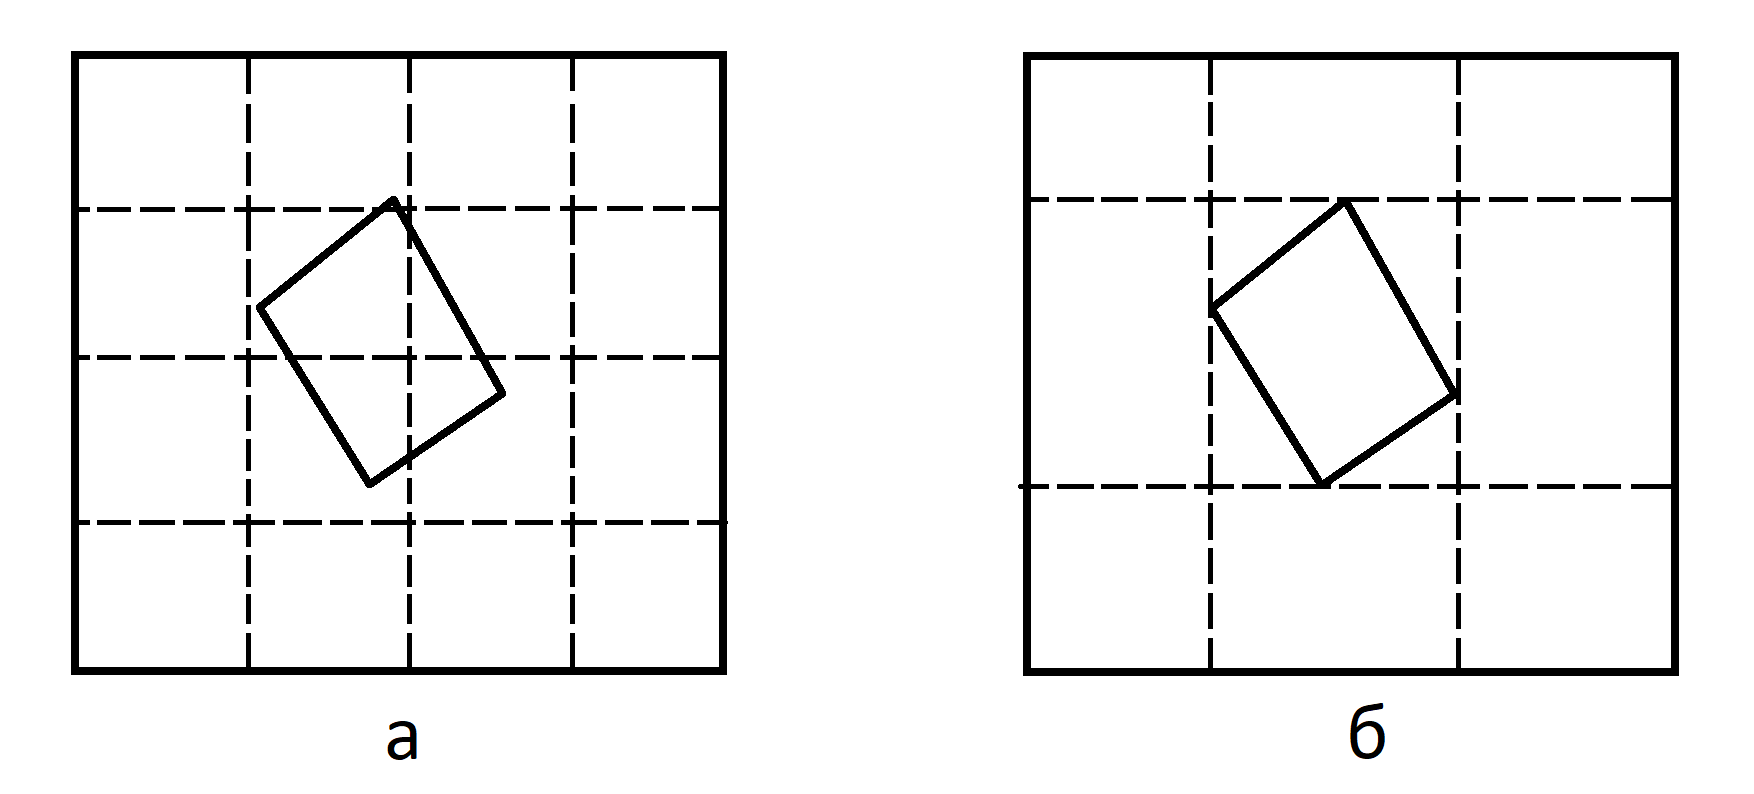
\includegraphics[width=\textwidth ]{img/subdivide.png}
	\caption{Сравнение двух способов разбиения окна}
\end{figure} 

Также в целях оптимизации можно выполнять предварительную сортировку многоугольников по глубине с целью оптимизации поиска многоугольников, охватывающих рассматриваемое окно.

Стоит отметить, что рекурсивное разбиение окна, в зависимости от числа пересечений объектов, может стать как положительной, так и отрицательной стороной алгоритма Варнока. Чем меньше пересечений объектов сцены, тем быстрее выполнится алгоритм.

\subsection{Алгоритм Вейлера-Азертона}
В алгоритме Вейлера-Азертона  производится попытка минимизировать количество шагов в алгоритме Варнока путем разбиения окна вдоль границ многоугольника.

Алгоритм решения задачи удаления невидимых линий и поверхностей удаления целиком базируется на алгоритме отсечения тех же авторов. Работа будет вестись с проекциями многоугольников, то есть в пространстве изображения. Алгоритм отсечения позволяет найти как внутренние, так и внешние отсечения, что важно.

Основные этапы алгоритма Вейлера-Азертона:
\begin{enumerate}
	\item[1)] сортировка многоугольников по глубине;
	\item[2)] отсечение всех многоугольников сцены по границе ближайшего к наблюдателю многоугольника;
	\item[3)] удаление многоугольников, экранируемых ближайшим к наблюдателю многоугольником;
	\item[4)] рекурсивное разбиение многоугольников, выполняемое в том случае, когда многоугольники, расположенные в списке за ближайшим многоугольником.
\end{enumerate}

К недостаткам алгоритма можно отнести то, что он не справляется с ситуацией пересечения двух многоугольников, поэтому в нём приходится отдельно рассматривать этот случай и разбивать один из них по линии пересечения многоугольников.

Ввиду больших затрат времени и памяти на выполнение алгоритма отсечения Вейлера-Азертона, основанного на работе с двунаправленными циклическими списками, соответствующий алгоритм удаления невидимых линий и поверхностей нельзя считать более эффективным, чем алгоритм Варнока.

\subsection{Алгоритм, использующий Z-буфер}
Алгоритм, использующий Z-буфер является одним из простейших алгоритмов удаления невидимых поверхностей, который работает в пространстве изображения.

Для своей работы он использует два буфера: буфер кадра, хранящий цвет (интенсивность) каждого пикселя в пространстве изображения, и Z-буфер (буфер глубины), хранящий информацию о координате Z для каждого пикселя. Вначале в Z-буфер заносятся минимальные значения Z, а буфер кадра заполняется фоновыми значениями. Затем каждый многоугольник преобразуется в растровую форму и записывается в буфер кадра, при этом не производится начального упорядочения.

В процессе работы глубина (значение координаты Z) каждого нового пикселя, который надо занести в буфер кадра, сравнивается с глубиной того пикселя, который уже занесён в Z -буфер. Если это сравнение показывает, что новый пиксель расположен ближе к наблюдателю, чем пиксель, уже находящийся в буфере кадра, то новый пиксель заносится в буфер кадра. Кроме того, производится корректировка Z-буфера: в него заносится глубина нового пикселя. Если же глубина рассматриваемого пикселя меньше глубины пикселя, хранящегося в Z-буфере, то никаких действий производить не надо.

Достоинства:
\begin{itemize}
	\item простота визуализации сцен любой сложности;
	\item отсутствие сортировки объектов сцены по глубине, как в других алгоритмах.
\end{itemize}

Недостатки:
\begin{itemize}
	\item большой объём задействуемой памяти;
	\item трудоёмкость устранения лестничного эффекта;
	\item трудоёмкость реализации эффектов, связанных с полупрозрачностью просвечиванием и рядом других специальных задач, повышающих реалистичность изображения.
\end{itemize}

Последний недостаток связан с тем, что пиксели заносятся в буфер кадра в произвольном порядке. Это затрудняет получение информации, необходимой для методов, основывающихся на предварительном анализе изображения. Проблема относительно легко решается использованием методов постфильтрации.

Ввиду того, что алгоритм требует объём памяти, в разы превышающий тот, который имеют микроконтроллеры семейства STM32, его рассмотрение для реализации поставленной задачи не имеет смысла.

\subsection{Алгоритм построчного сканирования, использующий Z-буфер}
Использование методов построчного сканирования в алгоритме, использующем Z-буфер, решается проблема использования большого количества памяти за счёт того, что буферизуется не экран, а только одна сканирующая строка.

Алгоритмы построчного сканирования работают в пространстве изображения и обрабатывают сцену в порядке прохождения сканирующей строки. Для каждого пикселя вычисляется глубина многоугольника, пересекающего рассматриваемую сканирующую строку. 

Количество вычислениий можно сократить, если использовать понятие интервалов. Решение задачи удаления невидимых поверхностей сводится к выбору видимых отрезков в каждом интервале, полученном путём деления сканирующей строки проекциями точек пересечения рёбер.

За то, что алгоритм построчного сканирования, использующий Z-буфер, решает проблему большого расхода памяти, приходится расплачиваться дополнительными вычислениями, связанными с использованием списка активных многоугольников.

\subsection{Алгоритм, использующий список приоритетов}
В основе алгоритма лежит сортировка объектов по приоритету, то есть по глубине объектов сцены или их расстоянию от точки наблюдения. Сначала изображаются объекты, расположенные дальше всех от наблюдателя, а затем их перекрывают объекты, находящиеся ближе к наблюдателю.

После сортировки объектов сцены по глубине и получается первоначальный список приоритетов. Далее он корректируется путём выполнения серии тестов на экранирование для каждой пары многоугольников в списке. Эти тесты достаточно трудоёмкие с точки зрения эффективности по времени и сложности реализации.

Также стоит отметить, что в алгоритме очень сложно идентифицируются случаи пересечения и циклического перекрытия многоугольников сцены.

\subsection{Алгоритм определения видимых поверхностей путем трассировки лучей}
В алгоритме, использующем трассировку лучей, отслеживаются (трассируются) лучи, идущие от наблюдателя к объекту. Такая трассировка называется обратной.

Для определения видимых поверхностей от наблюдателя, находящегося в бесконечности на положительном направлении оси Z, испускаются лучи, проходящие через каждый пиксель картинной плоскости. Траектория каждого луча отслеживается, чтобы определить пересечения объектов сцены с данным лучом. Пересечение с максимальным значением z представляет видимую поверхность для данного пикселя картинной плоскости.

\begin{figure}[h]
	\centering
	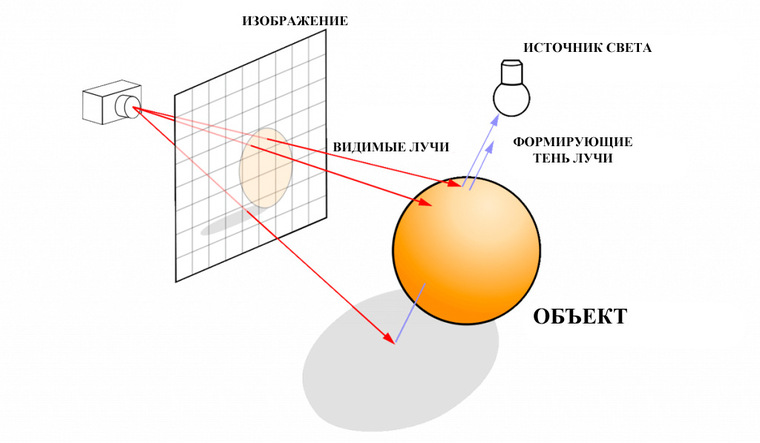
\includegraphics[width=\textwidth ]{img/raytracing.png}
	\caption{Иллюстрация алгоритма определения видимых поверхностей путем трассировки лучей}
\end{figure} 

Поиск пересечений является наиболее важным и трудоемким элементом этого алгоритма, поэтому его быстродействие существенно зависит от скорости их определения. Однако, несмотря на трудоёмкость этой процедуры, вычислительная сложность метода линейно зависит от количества объектов сцены. 

Главное преимущество алгоритма трассировки лучей – качество и реалистичность изображения. Также при использовании данного алгоритма нетрудно реализовать наложение света и тени на объекты.

К недостаткам данного алгоритма можно отнести производительность, так как трассировка большого количества лучей является очень трудоёмким процессом. Учёт прозрачности, усложняющий процесс трассировки лучей, только усугубит проблему.

\section{Анализ алгоритмов закрашивания}
\subsection{Простая закраска}
При использовании простой закраски вся грань многогранника закрашивается одним уровнем интенсивности, который вычисляется по закону Ламберта.

Предпосылки к использованию простой закраски:
\begin{enumerate}
	\item[1)] источник света находится на бесконечном удалении от объектов сцены;
	\item[2)] наблюдатель находится на бесконечном удалении от объектов сцены;
	\item[3)] закрашиваемая грань реально существует, а не является результатом аппроксимации другой поверхности.
\end{enumerate}

Из последнего пункта вытекает недостаток алгоритма простой закраски: он не подходит для закраски криволинейных поверхностей. Также к недостаткам алгоритма можно отнести то, что он никак не учитывает отражённый свет.

Главное преимущество алгоритма - простота реализации. Если поместить наблюдателя в бесконечность, то данный алгоритм хорошо подойдёт для решения поставленной задачи.

\subsection{Закраска по Гуро}
Закраска по Гуро предполагает билинейную интерполяцию интенсивностей. В результате вычисления интенсивности в каждой точке грани создаётся иллюзия гладкой криволинейной поверхности.

Закраска по Гуро хорошо сочетается с простой моделью освещения с диффузным отражением.

Несмотря на то, что применение закраски по Гуро сильно улучшает качество изображения, этот алгоритм имеет свои недостатки:
\begin{enumerate}
	\item[1)] появляется эффект полос Маха;
	\item[2)] в результате сглаживания теряется граница между гранями многогранника, что в некоторых случаях может дать неверный результат.
\end{enumerate}

Последний недостаток можно устранить, разбивая грани многогранника или создавая возмущения в уравнения нормалей к граням, чтобы сделать их разными. Однако такой подход увеличит объём вычислений.

\subsection{Закраска по Фонгу}
Закраска по Фонгу предполагает билинейную интерполяцию нормалей к граням многогранника. Такой подход требует больших вычислительных затрат, чем закраска по Гуро, и в результате даёт более качественное изображение, устраняя большинство недостатков предыдущего алгоритма.

\begin{figure}[h]
	\centering
	
\includegraphics[width=\textwidth ]{img/shading.png}
	\caption{Сравнение методов закраски: слева – простая, в центре – Гуро, справа – Фонга}
\end{figure}

К недостаткам закраски по Гуро и по Фонгу можно отнести ошибки при закраске невыпуклых многоугольников, а также большую вычислительную сложность и ресурсоёмкость.

\section{Вывод из аналитического раздела}
В данном разделе были проанализированы перспективы работы с семейством STM32, существующие решения поставленной задачи, а также методы моделирования трёхмерных объектов. Ввиду отсутствия универсальных программных инструментов для платформы STM32, которые могли бы решать задачи трёхмерной компьютерной графики, а также с учётом переносимости программного обеспечения на отечественные платформы, разработка имеет актуальность.

Несмотря на перспективы импортозамещения, для разработки была выбрана оригинальная платформа STM32 ввиду её более развитой экосистемы и наличия большого количества материалов по работе с микроконтроллерами этого семейства. Это упростит работу с микроконтроллером и его периферийными устройствами, а также разработку программных продуктов для данной платформы, что позволит уделить больше внимания задачам компьютерной графики.

В качестве алгоритма удаления невидимых линий и поверхностей был выбран алгоритм Варнока ввиду его компактности и относительно небольшой вычислительной сложности, а в качестве алгоритма закраски -  простая закраска по причине её относительно небольшой ресурсоёмкости и вычислительной сложности.




%%% Local Variables:
%%% mode: latex
%%% TeX-master: "rpz"
%%% End:

\chapter{Конструкторский раздел}
\label{cha:design}

В данном разделе будут описаны особенности аппаратной платформы STM32, а также алгоритмы и структуры данных, выбранные для решения 
поставленной задачи, будет разработана структура программного комплекса.

\section{Особенности архитектуры ARM}

\textbf{Архитектура ARM} — система команд и семейство описаний и готовых топологий 32-битных и 64-битных микропроцессорных/микроконтроллерных ядер.

Архитектура развивалась с течением времени и, начиная с ARMv7, были определены три профиля: для устройств, требующих высокой производительности (смартфоны, планшеты), для приложений, работающих в реальном времени, и для микроконтроллеров и бюджетных встраиваемых устройств. \cite{ARM_dev_doc}

Основные отличия архитектуры ARM от x86, которая используется в современных ПК: \cite{ARM_vs_x86}
\begin{itemize}
	\item использование упрощенного набора инструкций - \textbf{RISC} (Reduced Instruction Set Computing);
	\item предикация - возможность условного исполнения практически любой команды;
	\item упрощённая работа с памятью за счёт использования единого адресного пространства для всех устройств вычислительной машины;
	\item более объёмная регистровая архитектура; \cite{ARM_registers} \cite{x86_registers}
	\item меньшее энергопотребление;
	\item системы, базирующиеся на процессорах ARM, проще масштабировать и отлаживать;
\end{itemize}

Архитектура ARM поддерживается множеством операционных систем, к числу которых относятся Linux (в том числе Android, основанная на ядре ОС Linux), iOS, BSD, macOS Big Sur. Также на платформе запускаются отдельные варианты семейства ОС Windows: Windows CE, Windows Phone, Windows RT, Windows 10.

Процессоры ARM широко используются в потребительской электронике, к которой относятся смартфоны, плееры, портативные игровые консоли, калькуляторы, умные часы и компьютерные периферийные устройства. Эти процессоры имеют низкое энергопотребление, поэтому находят широкое применение во встраиваемых системах и преобладают на рынке мобильных устройств, для которых данный фактор критически важен. \cite{ARM_consumers}

\section{Описание семейства микроконтроллеров STM32}
Многие лицензиаты готовых топологий ядер ARM проектируют собственные топологии ядер на базе системы команд ARM. Одной из таких компаний является STMicroelectronics, производящая различные полупроводниковые электронные и микроэлектронные компоненты, к которым относятся микроконтроллеры семейства STM32.

\textbf{STM32} — семейство микроконтроллеров, основанных на 32-битных ядрах ARM Cortex-M. Каждый микроконтроллер состоит из ядра процессора, статической RAM-памяти, флеш-памяти, отладочного и различных периферийных интерфейсов.

Дизайн ядра ARM имеет множество настраиваемых опций, и для каждого микроконтроллера выбирается индивидуальная конфигурация с добавлением своих собственных периферийных устройств к ядру микроконтроллера перед преобразованием дизайна в полупроводниковую пластину.

Основные преимущества микроконтроллеров STM32:
\begin{itemize}
	\item низкая стоимость;
	\item гибкая и масштабируемая экосистема;
	\item большой выбор сред разработки;
	\item высокая производительность;
	\item наличие инструментов для отладки микроконтроллера;
\end{itemize}

Самым важным преимуществом STM32 является взаимозаменяемость чипов, которая достигается за счёт универсальности ядра STM32, позволяющего менять производителя c минимальными затратами на программный код. Также внутри семейства STM32 поддерживается pin-to-pin совместимость, которая позволяет менять объем памяти (флэш-память и ОЗУ) и периферию (Ethernet, USB, CAN и так далее), не меняя печатную плату. Таким образом, если для решения какой-либо задачи не хватает ресурсов одного микроконтроллера, его можно заменить на более мощный, не меняя самой схемы и платы. \cite{STM32_advantages}

\section{Структуры данных}
Чтобы формализовать алгоритм синтеза изображения в программе, необходимо определить структуры данных, которые будут в ней использоваться. Итак, будем считать, что
\begin{enumerate}
	\item[1)] трёхмерные модели являются полигональными, тогда сцену можно представить в виде массива многоугольников (полигонов);
	\item[2)] многоугольник включает в себя следующие данные:
	\begin{itemize}
		\item количество вершин;
		\item массив x и y координат вершин;
		\item коэффициенты уравнения поверхности, несущей данный многоугольник, заданного в виде $a*x + b*y + c*z = 1000$;
		\item цвет;
	\end{itemize}
	\item[3)] окна, использующиеся в алгоритме Варнока, имеют прямоугольную форму и хранят следующую информацию:
	\begin{itemize}
		\item количество многоугольников, рассматриваемых при изображении данного окна;
		\item массив многоугольников;
		\item координаты x и y левой нижней и правой верхней вершин окна;
	\end{itemize}
\end{enumerate}

\section{Разработка алгоритмов}
\subsection{Алгоритм работы программы}
Диаграмма, оформленная в соответствии с нотацией IDEF0 и отражающая общую декомпозицию алгоритма работы программы, представлена в приложении \ref{cha:appendix1}.


\subsection{Алгоритм Варнока}

Для удаления невидимых линий и поверхностей был выбран алгоритм Варнока, основанный на рекурсивном разбиении окон. Под окном в данном алгоритме понимается область изображения на дисплее, которая может содержать визуализируемые объекты сцены. Разбиение окон в алгоритме Варнока может быть реализовано как рекурсивно, так и итерационно. В данной работе будет рассматриваться итерационная реализация с использованием стека окон, так как она задействует меньший объём памяти, чем рекурсивная. Максимальная длина стека окон составляет
\begin{equation}
]\log_{2} (max(w; h))[ + 2 * (]\log_{2} (min(w; h))[ + 1) + 2,
\label{F:F1}
\end{equation}
где w – горизонтальное разрешение дисплея, h – вертикальное разрешение дисплея.

Схема алгоритма Варнока представлена в приложении \ref{cha:appendix2} на рисунке \ref{fig:warnock_algorithm} На рисунке \ref{fig:warnock_identification} представлен алгоритм идентификации взаимного расположения окна и рассматриваемого многоугольника. Алгоритм следует оформить в виде подпрограммы.

\section{Структура программного комплекса}
На рисунке \ref{fig:deploy_diagram} представлена структура программного комплекса, оформленная в виде диаграммы развёртывания. Она отражает компоненты, необходимые для работы системы, а также способы их взаимодействия.

\begin{figure}[h]
	\centering
	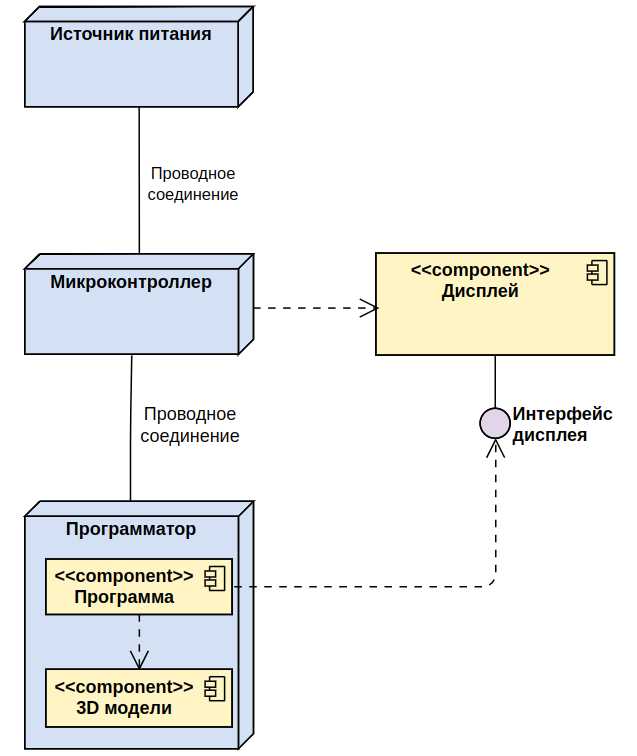
\includegraphics[scale=0.777 ]{img/deploy_diagram/dd1.png}
	\caption{Диаграмма развёртывания программного комплекса.}
	\label{fig:deploy_diagram}
\end{figure} 

\section{Вывод}
В данном разделе были описаны особенности работы с аппаратной платформой STM32, структура программного комплекса, а также алгоритмы и 
структуры данных, выбранные для решения поставленной задачи и отвечающие требованиям компактности, простоты и быстродействия.
%\begin{lstlisting}[style=pseudocode,caption={Алгоритм Флойда-Стейнберга и белый шум}]
%for x in range(width):
%    for y in range(height):
%        P(x,y) = trunc(I(x,y)+0.5)
%        e = I(x,y) - P(x,y)
%        I(x,y+1) += random.randint(1,alpha*16)/16*e
%        I(x+1, y-1) += random.randint(1,beta*16)/16*e
%        I(x+1, y) += random.randint(1,gamma*16)/16*e
%        I(x+1, y+1) +=  random.randint(1,sigma*16)/16*e
%\end{lstlisting}


%%% Local Variables:

%%% mode: latex
%%% TeX-master: "rpz"
%%% End:
%--количество цветов
%||количество пикселей
%\section{Выбор  языка программирования}
%Выбранный язык – С++.
%Причины:
%\begin{enumerate}
%	 \item Компилируемый язык со статической типизацией. 
%	 \item Сочетание высокоуровневых и низкоуровневых средств.
%	 \item Реализация ООП.
%	 \item Наличие удобной стандартной библиотеки шаблоны
%	 \end{enumerate}
%\section{Выбор вспомогательных библиотек}
%Для реализации программы была выбрана библиотека Qt.
%\begin{enumerate}
%	\item Широкие возможности работы с изображениями, в том числе и попиксельно
%	\item Наличии более функциональных аналогов стандартной библиотеки шаблонов в том числе для разнообразных структур данных
%\end{enumerate}
%\subsection{Диаграмма классов}
%\begin{figure}[h!]
%	\centering
%	\includegraphics[width=\textwidth]{img/diagramm.png}
%	\caption{Диаграмма классов}
%	\label{fig:spire03}
%\end{figure}

%%% Local Variables:
%%% mode: latex
%%% TeX-master: "rpz"
%%% End:

\chapter{Технологический раздел}

В данном разделе будут рассмотрены детали реализации программного комплекса, описанного в конструкторской части работы, и приведены примеры 
работы программы.

\section{Выбор и обоснование средств разработки}
В качестве языка программирования, на котором будет реализовано программное обеспечение, выбран язык C++ \cite{cpp}.
Данный выбор обусловлен следующими причинами:
\begin{enumerate}
	\item[1)] высокая скорость работы языка;
	\item[2)] строгая типизация;
	\item[3)] наличие библиотек для работы с микроконтроллерами семейства STM32 и периферийными устройствами;
	\item[4)] наличие большого количества материалов о разработке программного обеспечения для микроконтроллеров семейства STM32 на данном языке;
	\item[5)] возможность сертификации программ, написанных на данном языке \cite{fstec}.
\end{enumerate}

В качестве среды разработки был выбран текстовый редактор Visual Studio Code \cite{vscode}, обладающий большим количеством плагинов 
и инструментов для создания программного обеспечения на различных языках, в том числе на C++.

Для контроля качества кода использовался статический анализатор кода cppcheck \cite{cppcheck} и отладчик использования памяти 
valgrind \cite{valgrind}.



\section{Формат задания исходных данных}
Разработанный графический инструмент использует полигональное представление трёхмерных моделей. Для их задания необходима информация 
о полигонах, из которых состоит модель, а именно их геометрическое строение и цвет. Также для построения трёхмерной сцены необходима 
информация о расположении источников света.

\subsection{Задание геометрии трёхмерных моделей}
В качестве формата, задающего геометрическое строение и расположение полигонов на сцене, был выбран формат obj \cite{obj}. Это  простой 
формат данных, который представляет только трехмерную геометрию, а именно координаты вершин, индексы вершин, 
составляющие полигоны, а также текстуры и нормали. Важно заметить, что с форматом obj могут работать различные редакторы 
трёхмерной графики. Самыми популярными среди них являются Blender \cite{blender}, Autodesk AutoCAD \cite{autocad}, 
Adobe Photoshop \cite{photoshop} и КОМПАС-3D \cite{compass}. Пример файла формата obj приведён в приложении \ref{cha:appendix3} 
(листинг \ref{lst:cube_obj}).

\subsection{Задание характеристик материалов}
Формат obj помимо геометрии задаёт материалы, из которых выполнены заданные полигоны. Эти материалы подробно описывает формат 
mtl \cite{mtl}, который содержит в себе информацию о цвете и оптических свойствах полигонов, из которых состоит трёхмерная модель. 
Пример файла формата mtl приведён в приложении \ref{cha:appendix3} (листинг \ref{lst:cube_mtl}).

\subsection{Задание источников света}
Форматы obj и mtl описывают только трёхмерные модели не предусматривают задания расположения источников света на сцене. Поэтому 
для представления этих данных был разработан формат lgt, в котором построчно задаются вещественные координаты x, y, z источников света. 
Пример файла формата lgt приведён в приложении \ref{cha:appendix3} (листинг \ref{lst:cube_lgt}).



\section{Структура программы}
В программе реализованы следующие модули:
\begin{description}
	\item[reader] модуль чтения исходных данных из файлов;
	\item[converter] модуль подготовки исходных данных для алгоритмов визуализации;
	\item[writer] модуль записи сконвертированных данных в промежуточный файл;
	\item[display] модуль, предоставляющий данные о конкретном дисплее и функции для работы с ним;
	\item[errors] модуль обработки ошибок;
	\item[debug] отладочный модуль;
	\item[warnock] модуль, реализующий алгоритм Варнока удаления невидимых линий и поверхностей;
	\item[wstack] модуль, предоставляющий структуры данных "окно"{}, "стек окон"{} и операции над ними;
	\item[data\_structures] модуль, предоставляющий структуры данных, описывающие полигональные модели.
\end{description}

Диаграмма модулей программы представлена на рисунке \ref{fig:modules}.

\begin{figure}[h]
	\centering
	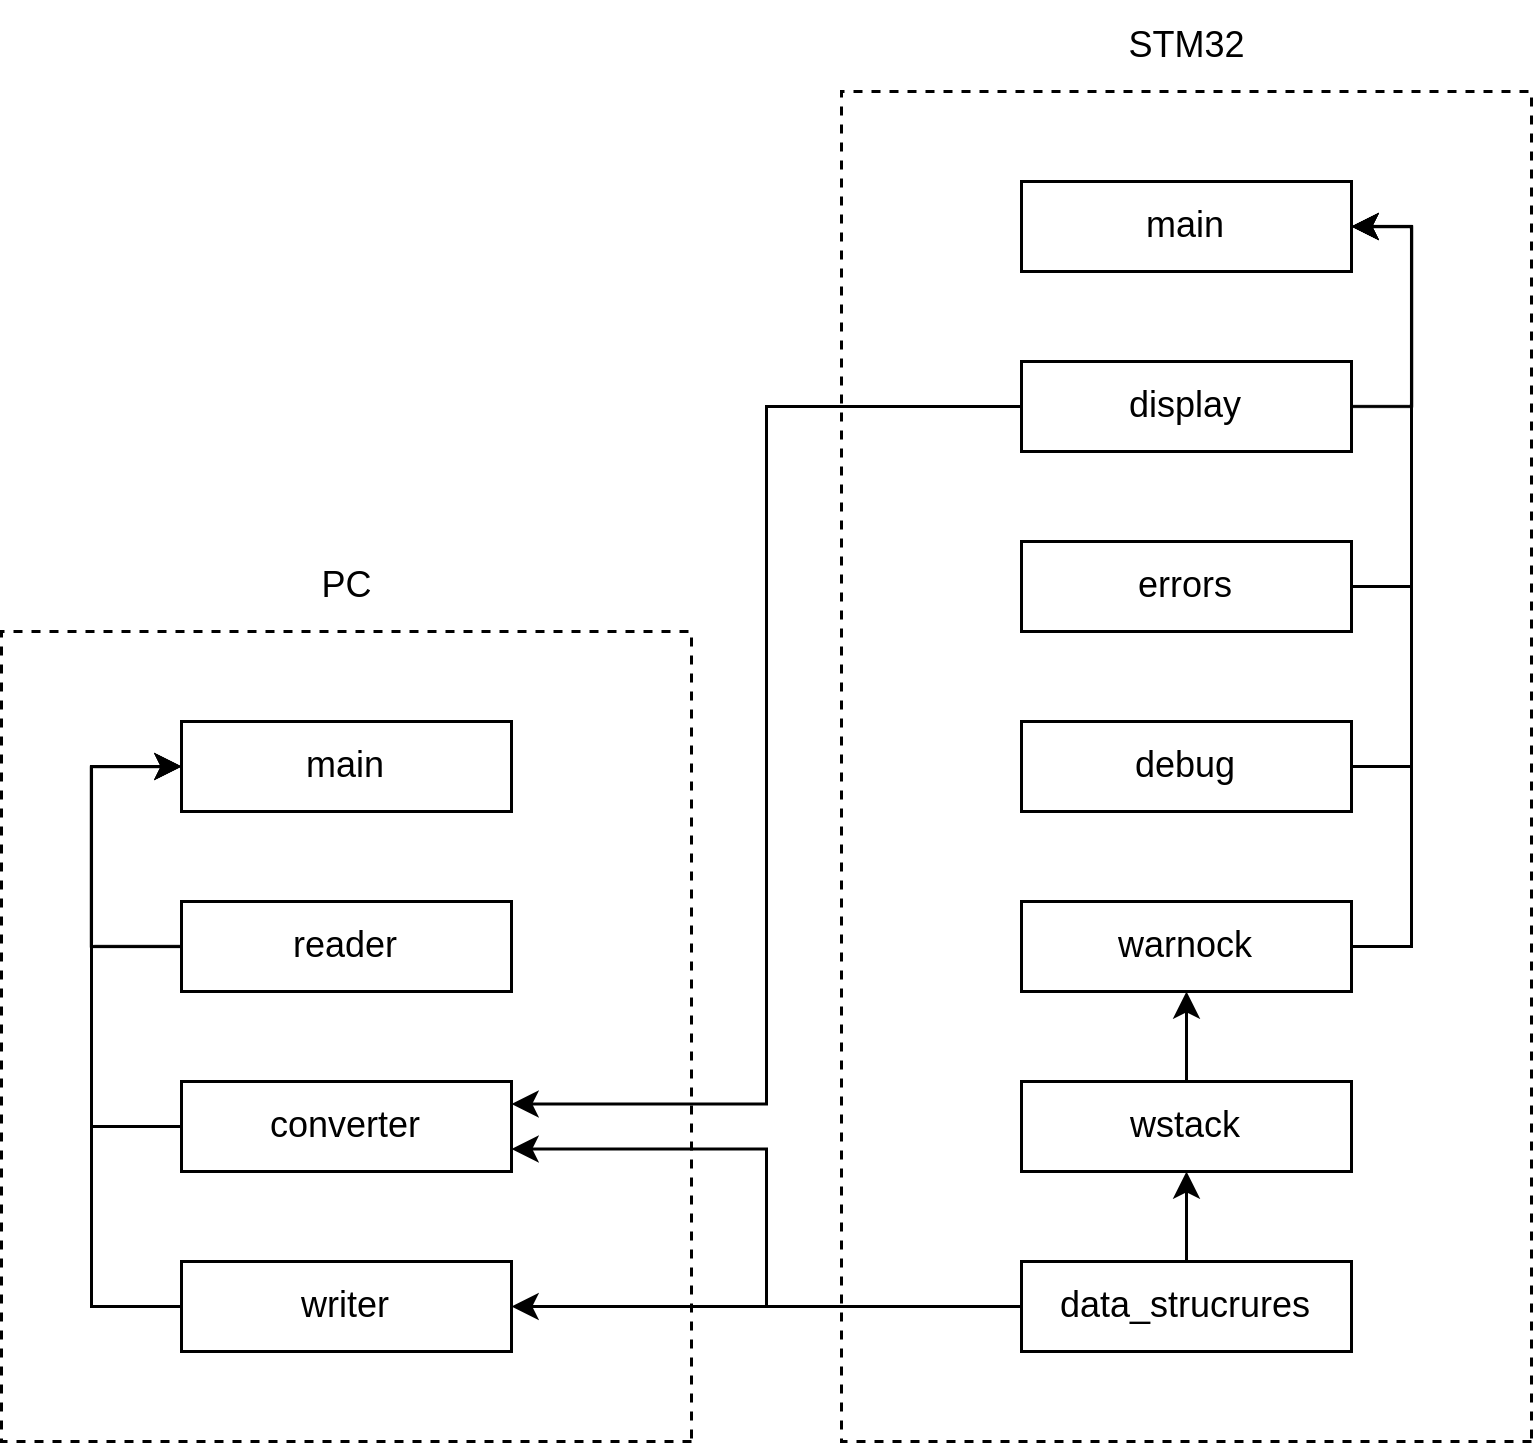
\includegraphics[width=\textwidth ]{img/modules/modules.png}
	\caption{Диаграмма модулей программы}
	\label{fig:modules}
\end{figure} 

Программа разделена на две части. Первая предназначена для предобработки исходных данных и выполняется на компьютере. Она получает на вход 
файлы с исходными данными и транслирует их в файл, который компонуется со второй частью программы, отвечающей за рендеринг изображения. 
Получившаяся программа загружается на микроконтроллер и выводит на дисплей заданное изображение.

Такая гибкая архитектура позволяет заменять аппаратное обеспечение, на котором должна выполняться программа, не затрагивая при этом 
алгоритмы рендеринга трёхмерной сцены. Это означает, что данное программное обеспечение обладает достаточно большой универсальностью
с точки зрения требований к аппаратному обеспечению и не зависит от конкретных моделей микроконтроллера и дисплея.

Также для развёртывания и запуска программы был написан сценарий сборки, предназначенный для запуска на операционных системах 
семейства Linux \cite{linux}.



\section{Детали реализации алгоритмов}
В листинге \ref{lst:warnock} представлен код функции warnock\_subdivide, которая реализует алгоритм Варнока удаления 
невидимых линий и поверхностей.
% \newpage
\lstinputlisting[language=C,caption=Алгоритм Варнока,label=lst:warnock]{listings/warnock.cpp}

Перед анализом каждого окна выполняется идентификация многоугольников с целью их разделения на три группы: внешние, 
охватывающие и все остальные. В том случае, если необходимо разбиение окна, оно делится на четыре равные части, если это возможно. 
Перед разбиением из массива многоугольников удаляются внешние, так как они заведомо будут внешними относительно подокон и 
не будут играть никакой роли при изображении сцены. Данная оптимизация повышает быстродействие алгоритма.

\section{Взаимодействие с программой}
Для программы был разработан консольный интерфейс, а не графический. Такое решение было принято по причине выбора формата задания 
исходных данных, не требующего от пользователя большого количества действий. Также консольный интерфейс позволяет использовать 
разработанный программный инструмент другими программами. В будущем это позволит разрабатывать программное обеспечение для семейства 
микроконтроллеров STM32, использующее трёхмерную графику.

Для запуска программы необходимо выполнить четыре шага: установить зависимости, подготовить исходные данные, подключить 
микроконтроллер к компьютеру и запустить рендеринг.

\subsection{Установка зависимостей}
Ввиду того, что для изменения выводимого на дисплей изображения программу приходится перекомпоновывать, на компьютере, с которого 
будет загружаться программа, должны быть установлены инструменты, необходимые для компоновки программы \cite{toolchain}. 
Также для запуска сценария сборки требуется утилита make \cite{make}.

\subsection{Подготовка исходных данных}
Рассмотрим данный и последующие этапы на примере модели куба. Для задания трёхмерных моделей необходимо создать 3 файла. 
Содержимое файлов cube.obj, cube.mtl и cube.lgt приведено в приложении \ref{cha:appendix3}. Первые два файла можно экспортировать 
из графических редакторов, а третий создать с помощью текстового редактора. Полученные файлы необходимо поместить в директорию 
проекта models/название\_модели (в примере директория будет называться models/cube).

\subsection{Подключение микроконтроллера}
Для загрузки программы на микроконтроллер необходимо подключить его к компьютеру с помощью проводного соединения и запомнить 
абсолютный путь к файлу устройства.

\subsection{Запуск программы}
Для запуска сборки необходимо выполнить в командной оболочке команду вида 
\lstinputlisting[language=bash,numbers=none]{listings/deploy.sh}
% \text{sudo make view model=cube device=/dev/sdb target=/run/media/inspirate/NODE\_F767ZI,}
где model - название модели, device - файл подключенного устройства, target - точка монтирования устройства. 
Далее произойдёт компиляция программы, после чего она загрузится на микроконтроллер и выведет изображение на дисплей. 



\section{Примеры работы программы}
На рисунке \ref{fig:cube} приведено изображение модели куба, рассматриваемое в качестве примера. Другие изображения моделей приведены в 
приложении \ref{cha:appendix4}.

\newpage
\begin{figure}[h]
	\centering
	\includegraphics[width=\textwidth ]{img/models/cube_with_hardware.jpg}
	\caption{Изображение модели куба на дисплее с разрешением 320x240 пикселей}
	\label{fig:cube}
\end{figure} 





\section{Вывод из технологического раздела}
В данном разделе были рассмотрены детали реализации программного инструмента, разработанного на основе алгоритма Варнока удаления 
невидимых линий и поверхностей. Также был рассмотрен алгоритм взаимодействия с программой и были приведены примеры её работы.

\chapter{Экспериментально-исследовательский раздел}
%\chapter{Заключение}
%\label{cha:research}

%В данном разделе проводятся вычислительные эксперименты.
%А на рис.~\ref{fig:spire01} показана схема мыслительного процесса автора...

%\begin{figure}
 % \centering
 % \caption{Как страшно жить}
 % \label{fig:spire01}
%\end{figure}

В данном разделе будет произведено исследование разработанного программного обеспечения с целью определения возможностей применения 
микроконтроллеров семейства STM32 для решения задач компьютерной графики.

\section{Цель проводимых измерений}
Для программы, которая должна выполняться на микроконтроллере, обладающем сравнительно небольшой вычислительной мощностью, критически 
важен фактор быстродействия. Особенно он важен при изображении сцены, содержащей большое количество объектов. В связи с этим очень 
важно понимать, как оборудование, исполняющее разработанную программу, будет справляться с увеличением нагрузки и как при этом 
будет изменяться ресурсоёмкость реализованных алгоритмов.

Целью проводимых измерений будет проведение нагрузочного тестирования и установление зависимости между числом объектов на сцене и затратами 
времени и памяти на работу алгоритма визуализации.



\section{Описание проводимых измерений}
Для установления зависимости между числом объектов на сцене и временем работы алгоритма будут произведены замеры времени при 
визуализации трёх моделей, содержащих 312, 1172 и 6228 полигонов. Изображения моделей приведены в приложении \ref{cha:appendix4}. 
В самом начале будет произведён замер времени визуализации небольшой части модели, а затем к ней постепенно будут добавляться 
новые полигоны до тех пор, пока число изображаемых полигонов не достигнет числа полигонов во всей модели и она не будет 
полностью изображена. Время будет замеряться в тактах процессора. Время высвечивания пикселей на дисплее учитываться не будет.

Замеры объёма памяти, необходимого для работы программы, будут произведены аналогично замерам времени, то есть путём исследования 
процесса визуализации отдельных фрагментов изображения. В процессе визуализации каждого фрагмента будет фиксироваться максимальный 
объём затраченной оперативной памяти. В этот объём входят данные об изображаемых моделях, а также статическая и динамическая память, 
используемая программой в процессе выполнения. Объём скомпилированного кода программы учитываться не будет, так как он хранится 
не в оперативной, а в постоянной памяти микроконтроллера.

Для проведения измерений будет использоваться модель микроконтроллера STM32F767ZI \cite{STM32F767ZI}, обладающая следующими 
техническими характеристиками:
\begin{itemize}
	\item модель процессора - Arm Cortex-M7 \cite{cortex_m7};
	\item тактовая частота процессора - 216 МГц;
	\item объём флеш-памяти - 2 Мб;
    \item объём оперативной памяти - 512 Кб.
\end{itemize}

Для просмотра получившихся изображений будет использоваться TFT-дисплей с разрешением 320x240 пикселей на базе чипа ILI9341 \cite{ili9341}.



\section{Инструменты измерения времени работы программы}
Для измерения реального времени процессора, затраченного на выполнение алгоритма визуализации трёхмерной сцены, будет использоваться 
отладочный модуль DWT \cite{dwt}. Данный модуль предосталяет функционал для профилирования работы процессора, в частности для замера 
количества тактов процессора, прошедших с момента начала работы программы.



\section{Результаты проведённых измерений}
Результаты измерений времени представлены на рисунке \ref{fig:measuring_time}.

% \begin{figure}[h]
%     \centering
%     \begin{subfloat}
%     {
%         \centering
        
%     }
%     \end{subfloat}
%     \hspace{10pt}       
%     \begin{subfloat}
%     {
%         \centering
        
%     }       
%     \end{subfloat}
%     \caption{Модель №1 (312 полигонов).}
%     \label{fig:tree_benchmark}
% \end{figure}

% \begin{figure}[h]
%     \centering
%     \begin{subfloat}
%     {
%         \centering
        
%     }
%     \end{subfloat}
%     \hspace{10pt}       
%     \begin{subfloat}
%     {
%         \centering
        
%     }       
%     \end{subfloat}
%     \caption{Модель №2 (1172 полигона).}
%     \label{fig:car_benchmark}
% \end{figure}

\begin{figure}[h]
    \centering
    \begin{subfloat}[Модель №1 (312 полигонов)]
    {
        \centering
        \begin{tikzpicture}
            \begin{axis}[width=0.47\textwidth, height=0.28\textheight,
                         xlabel={Количество полигонов},
                         ylabel={Количество тактов процессора}]
            \addplot table [x=count,y=cycles] {chart_tables/tree_time.txt};
            \end{axis}
        \end{tikzpicture}
    }
    \end{subfloat}
    \hspace{10pt}       
    \begin{subfloat}[Модель №2 (1172 полигона)]
    {
        \centering
        \begin{tikzpicture}
            \begin{axis}[width=0.46\textwidth, height=0.28\textheight,
                         xlabel={Количество полигонов},
                         ylabel={Количество тактов процессора}]
            \addplot table [x=count,y=cycles] {chart_tables/car_time.txt};
            \end{axis}
        \end{tikzpicture}
    }       
    \end{subfloat}
    \hspace{10pt}       
    \begin{subfloat}[Модель №3 (6228 полигонов)]
    {
        \centering
        \begin{tikzpicture}
            \begin{axis}[width=0.46\textwidth, height=0.28\textheight,
                         xlabel={Количество полигонов},
                         ylabel={Количество тактов процессора}]
            \addplot table [x=count,y=cycles] {chart_tables/plant_time.txt};
            \end{axis}
        \end{tikzpicture}
    }       
    \end{subfloat}
    \caption{Затраты времени на выполнение алгоритма визуализации}
    \label{fig:measuring_time}
\end{figure}

\newpage
Результаты измерений объёма памяти, необходимого программе, представлены на рисунке \ref{fig:measuring_memory}.

\begin{figure}[h]
    \centering
    \begin{subfloat}[Модель №1 (312 полигонов)]
    {
        \centering
        \begin{tikzpicture}
            \begin{axis}[width=0.47\textwidth, height=0.28\textheight,
                         xlabel={Количество полигонов},
                         ylabel={Объём памяти, Кб}]
            \addplot table [x=count,y=kilobytes] {chart_tables/tree_memory.txt};
            \end{axis}
        \end{tikzpicture}
    }
    \end{subfloat}
    \hspace{10pt}       
    \begin{subfloat}[Модель №2 (1172 полигона)]
    {
        \centering
        \begin{tikzpicture}
            \begin{axis}[width=0.46\textwidth, height=0.28\textheight,
                         xlabel={Количество полигонов},
                         ylabel={Объём памяти, Кб}]
            \addplot table [x=count,y=kilobytes] {chart_tables/car_memory.txt};
            \end{axis}
        \end{tikzpicture}
    }       
    \end{subfloat}
    \hspace{10pt}       
    \begin{subfloat}[Модель №3 (6228 полигонов)]
    {
        \centering
        \begin{tikzpicture}
            \begin{axis}[width=0.46\textwidth, height=0.28\textheight,
                         xlabel={Количество полигонов},
                         ylabel={Объём памяти, Кб}]
            \addplot table [x=count,y=kilobytes] {chart_tables/plant_memory.txt};
            \end{axis}
        \end{tikzpicture}
    }       
    \end{subfloat}
    \caption{Затраты памяти на выполнение алгоритма визуализации}
    \label{fig:measuring_memory}
\end{figure}



\newpage
\section{Вывод из экспериментально-исследовательского раздела}
В данном разделе было проведено исследование зависимости между числом объектов на сцене и ресурсоёмкостью алгоритма визуализации.

Результаты измерений показали, что зависимость затрат памяти на работу алгоритма от числа объектов на сцене является линейной. 
А зависимость затрат времени, предположительно, является кусочно-линейной. Коэффициент пропорциональности между числом объектов на сцене 
и временем работы алгоритма не является одинаковым на различных участках графиков, так как различные случаи взаимного расположения 
полигонов обрабатываются с разной скоростью. Увеличение времени работы алгоритма при добавлении на сцену очередного полигона зависит от 
того, будет ли он пересекаться с полигонами, которые уже находятся на сцене.

Также проведённые измерения показали, что оборудование, исполняющее разработанную программу, равномерно справляется с большой нагрузкой, 
так как зависимость между числом объектов на сцене и ресурсоёмкостью алгоритма является линейной на всех участках графиков. По результатам 
тестов, максимальное количество объектов (полигонов), которое микроконтроллер семейства STM32 позволяет обработать, превышает 6000.

%%% Local Variables:
%%% mode: latex
%%% TeX-master: "rpz"
%%% End:

%\chapter{Организационно-экономический раздел}
%\label{cha:econom}
%%% Local Variables:
%%% mode: latex
%%% TeX-master: "rpz"
%%% End:

%\chapter{Промышленная экология и %езопасность}\label{cha:bzd}


%%% Local Variables:
%%% mode: latex
%%% TeX-master: "rpz"
%%% End:


\backmatter %% Здесь заканчивается нумерованная часть документа и начинаются ссылки и
            %% заключение

\Conclusion % заключение к отчёту
В рамках курсового проекта был реализован программный инструмент для микроконтроллеров семейства STM32, который позволяет 
визуализировать трёхмерные модели.

Были рассмотрены существующие алгоритмы удаления невидимых линий и поверхностей и алгоритмы закраски, проанализированы 
их достоинства, недостатки и возможность использования для решения поставленной задачи. С учётом её особенностей были 
разработаны структуры данных для реализации выбранных алгоритмов.

Разработанная программа позволяет получать на экране дисплея изображение полигональной модели, заданной пользователем. При 
разработке были учтены недостатки существующих программных решений для аппаратной платформы STM32.

В ходе выполнения экспериментальной части работы было установлено, что разработанное программное обеспечение на тестовом оборудовании 
показывает высокую стабильность. При возрастании нагрузки на систему сохраняются эффективность работы программы и качество получаемого 
результата. Микроконтроллеры семейства STM32 подходят для решения относительно простых задач компьютерной графики, не требующих 
построения реалистических изображений с определением проекционных теней, использованием глобальной модели освещения и методов закраски, 
требующих больших вычислительных затрат.

Графический инструмент, разработанный в рамках курсового проекта, имеет по меньшей мере два направления дальнейшего развития.
\begin{enumerate}
	\item[1.] Разработка новых приложений, использующих разработанный графический инструмент. К этому располагают интерфейс программы и формат задания исходных данных.
	\item[2.] Перенос разработок с STM32 на отечественные аппаратные платформы. Это возможно благодаря наличию аналогов семейства микроконтроллеров STM32 отечественного производства.
\end{enumerate}

%\begin{figure}
%	За практику я смог рассмотреть и попробовать полный процесс подготовки к разработке законченного программного продукта, а именно составить техническое задание, провести анализ алгоритмов и методов решения поставленной задачи, составить диаграмму классов и примерный каркас программы. Так же были получены первые результаты работы программы- а именно "зашумленные" при помощи дизеринга картинки.
%\end{figure}
%%% Local Variables: 
%%% mode: latex
%%% TeX-master: "rpz"
%%% End: 


% % Список литературы при помощи BibTeX
% Юзать так:
%
% pdflatex rpz
% bibtex rpz
% pdflatex rpz

\bibliographystyle{ugost2008}
\bibliography{rpz}


%%% Local Variables: 
%%% mode: latex
%%% TeX-master: "rpz"
%%% End: 


\appendix   % Тут идут приложения

\chapter{IDEF0-диаграмма алгоритма работы программы}
\label{cha:appendix1}

\begin{figure}[h]
	\centering
	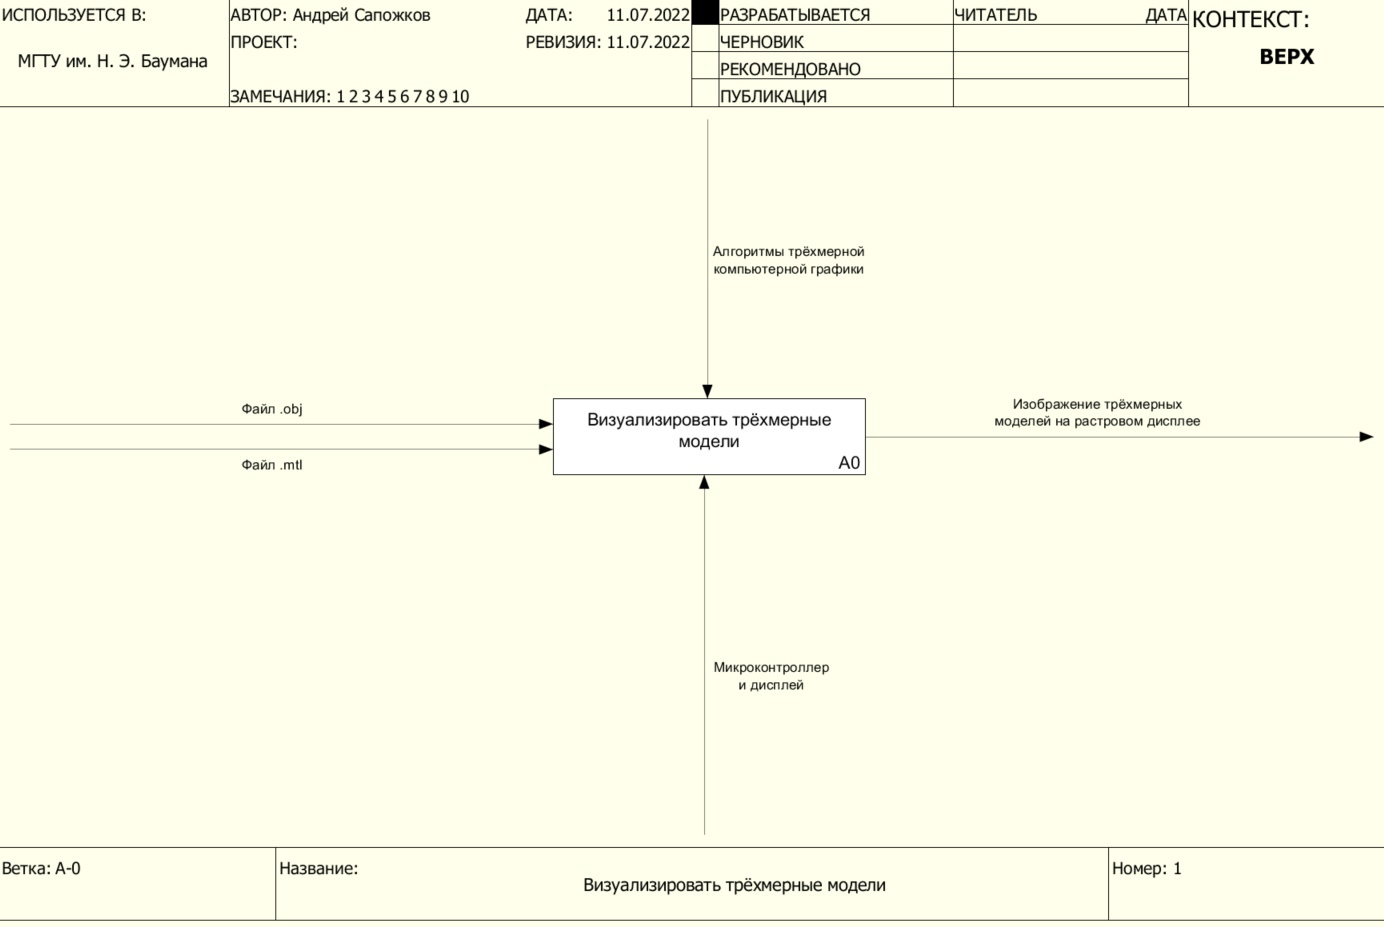
\includegraphics[width=\textwidth ]{img/IDEF0/A0.jpg}
	\caption{Верхний уровень диаграммы.}
\end{figure} 

\begin{figure}[h]
	\centering
	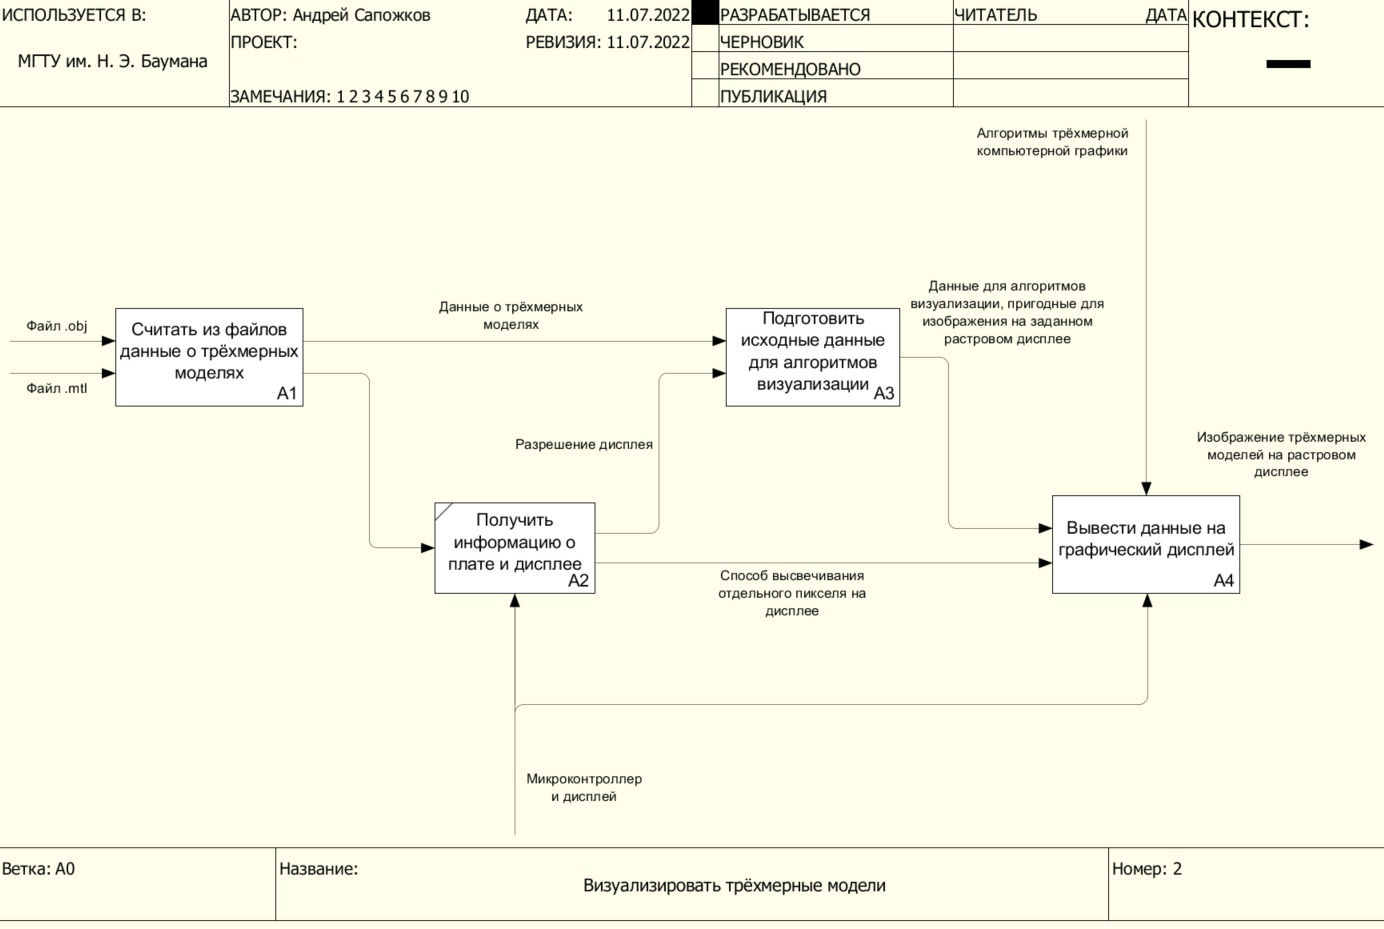
\includegraphics[width=\textwidth ]{img/IDEF0/A0_decomposition.jpg}
	\caption{Декомпозиция уровня A0.}
\end{figure} 

\begin{figure}[h]
	\centering
	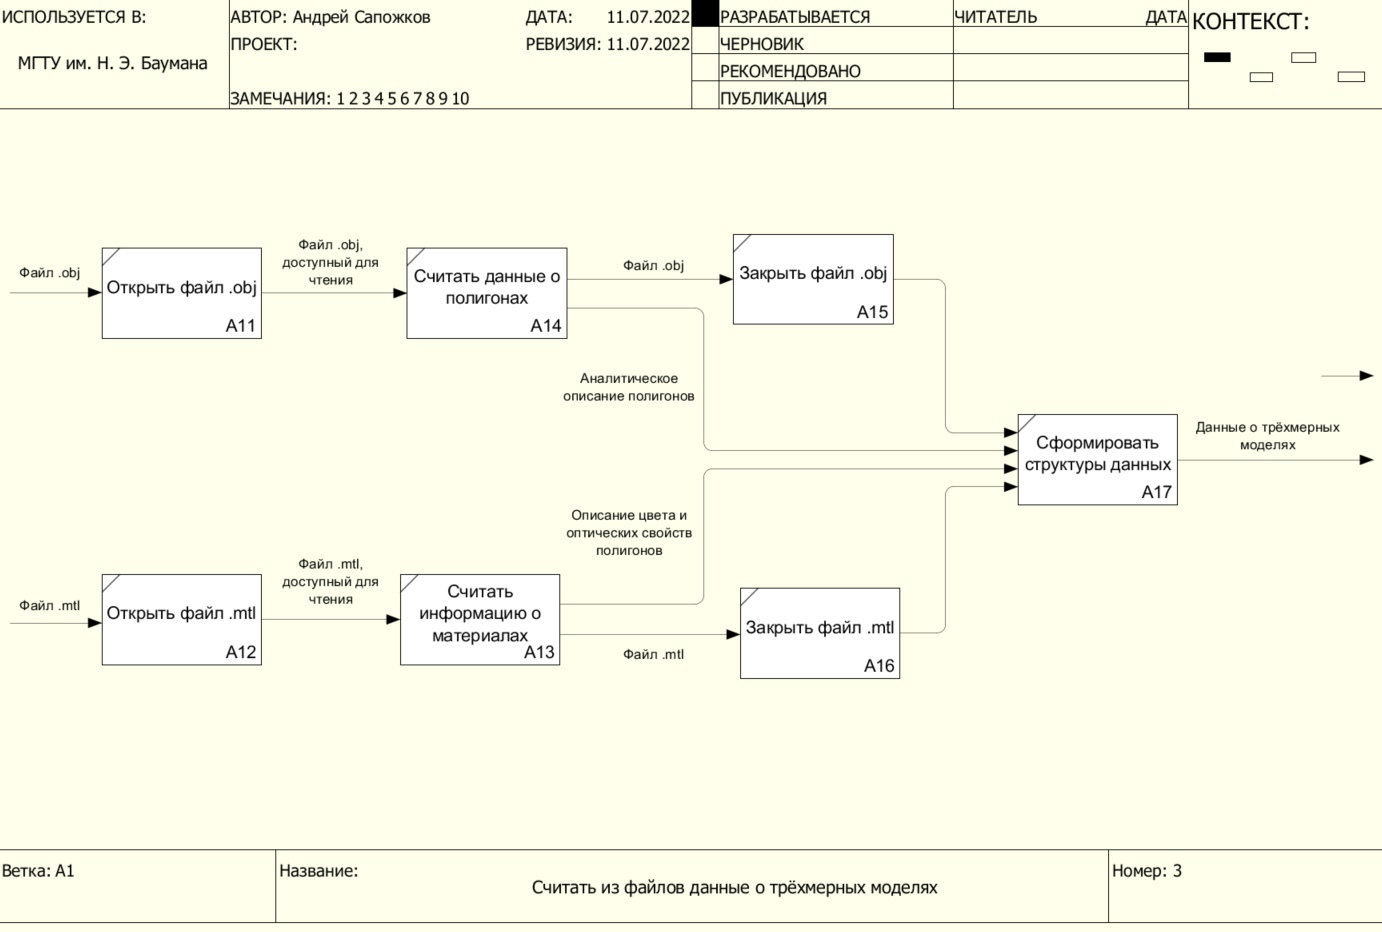
\includegraphics[width=\textwidth ]{img/IDEF0/A1_decomposition.jpg}
	\caption{Декомпозиция уровня A1.}
\end{figure} 

\begin{figure}[h]
	\centering
	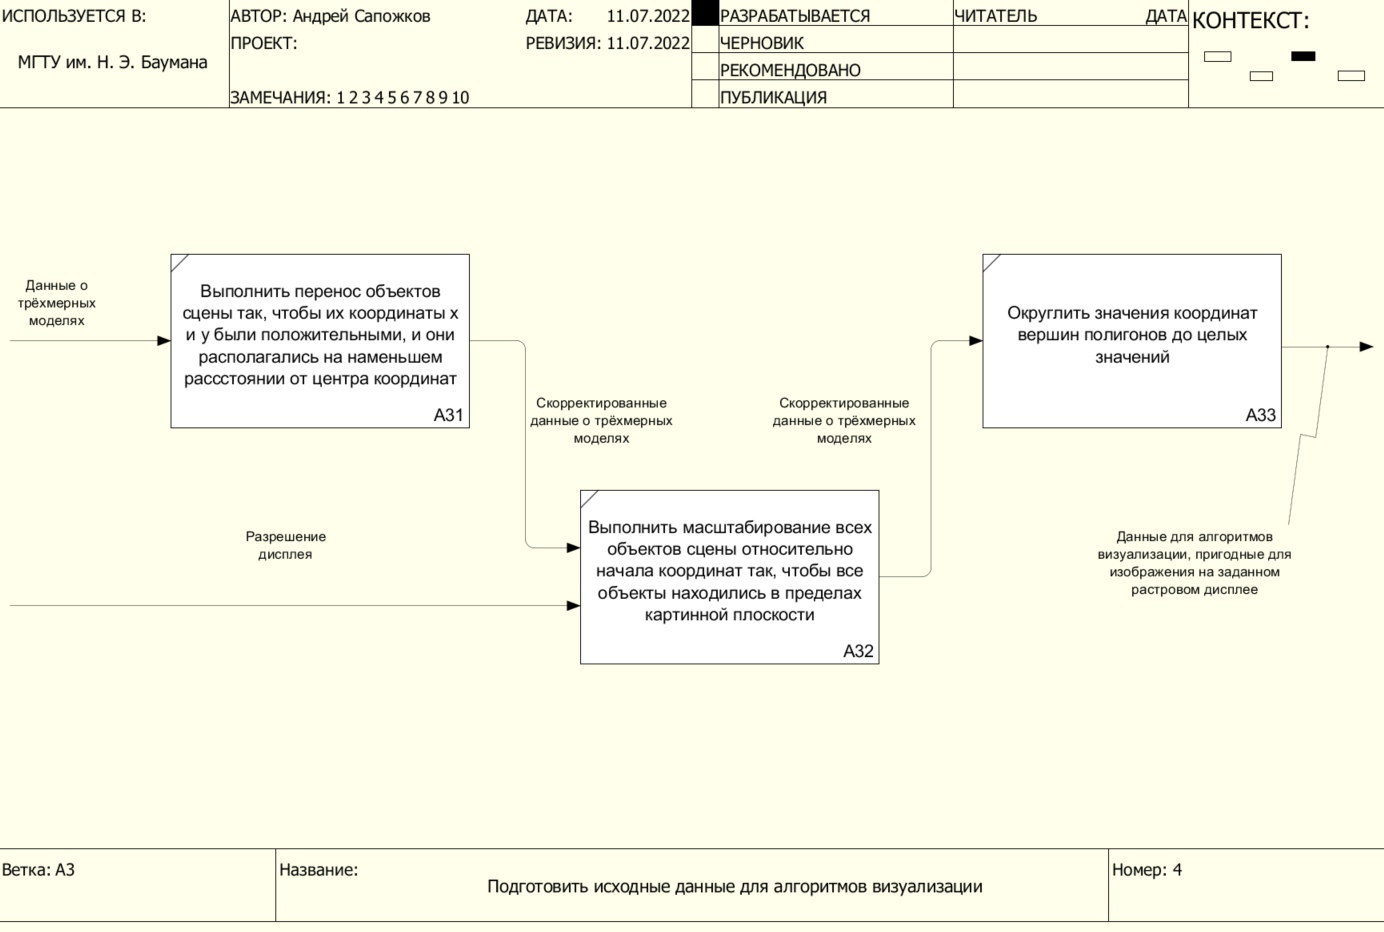
\includegraphics[width=\textwidth ]{img/IDEF0/A3_decomposition.jpg}
	\caption{Декомпозиция уровня A3.}
\end{figure} 

\begin{figure}[h]
	\centering
	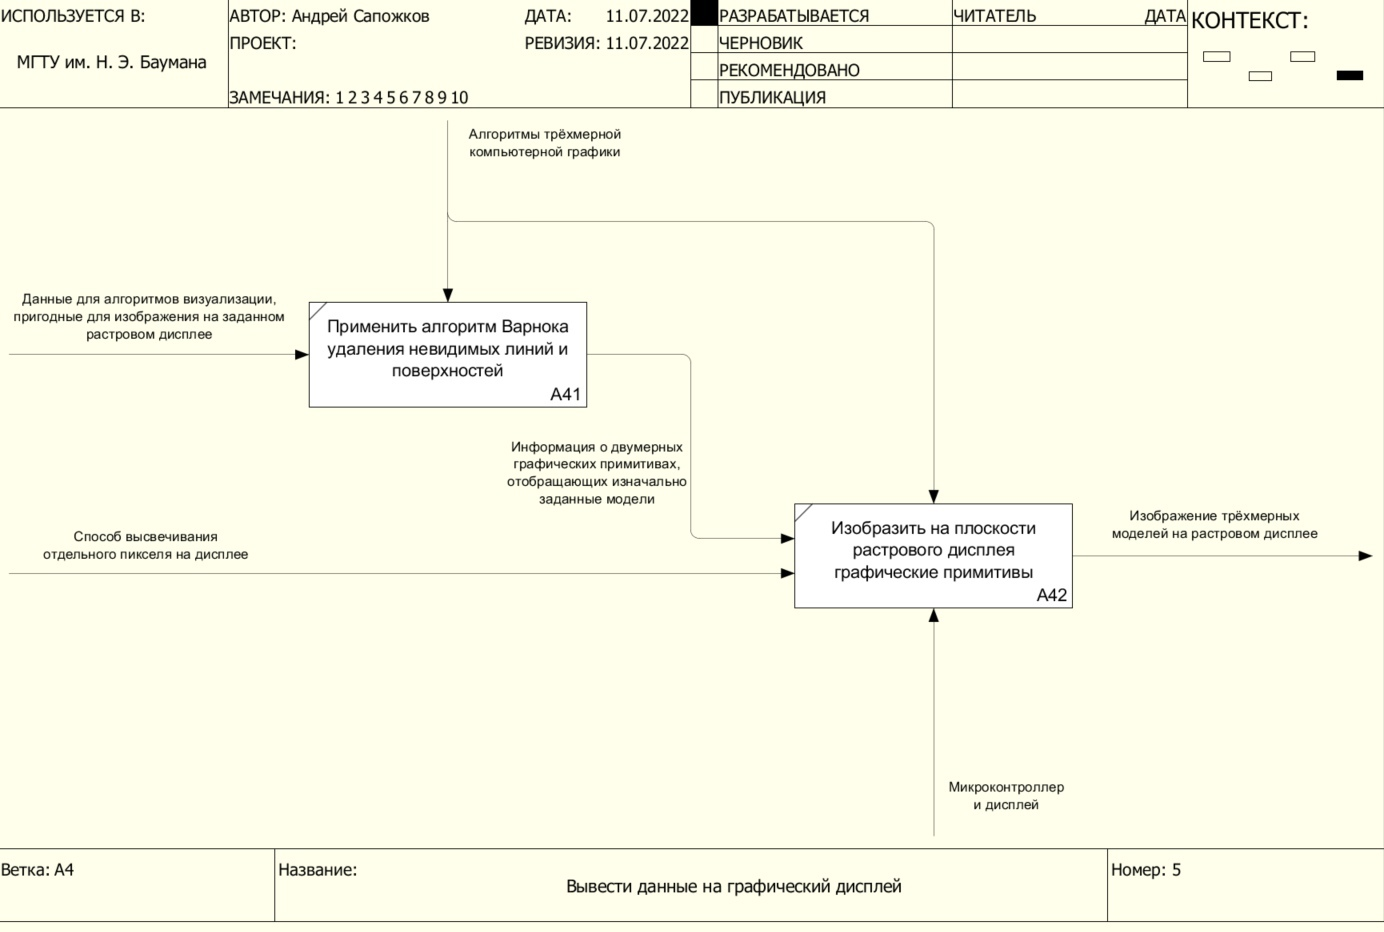
\includegraphics[width=\textwidth ]{img/IDEF0/A4_decomposition.jpg}
	\caption{Декомпозиция уровня A4.}
\end{figure} 

%%% Local Variables: 
%%% mode: latex
%%% TeX-master: "rpz"
%%% End: 

\chapter{Вывод формулы максимального размера стека окон в Алгоритме Варнока}
\label{cha:appendix2}

Пусть выполняется рекурсивное разбиение окна на четыре равные части, причём сначала оно разбивается по стороне с максимальной длиной, а затем по стороне с минимальной длиной. Разбиение производится, если длина соответствующей стороны окна больше 1. На рисунке \ref{fig:subdivide_2} показаны примеры таких разбиений.

\begin{figure}[h]
	\centering
	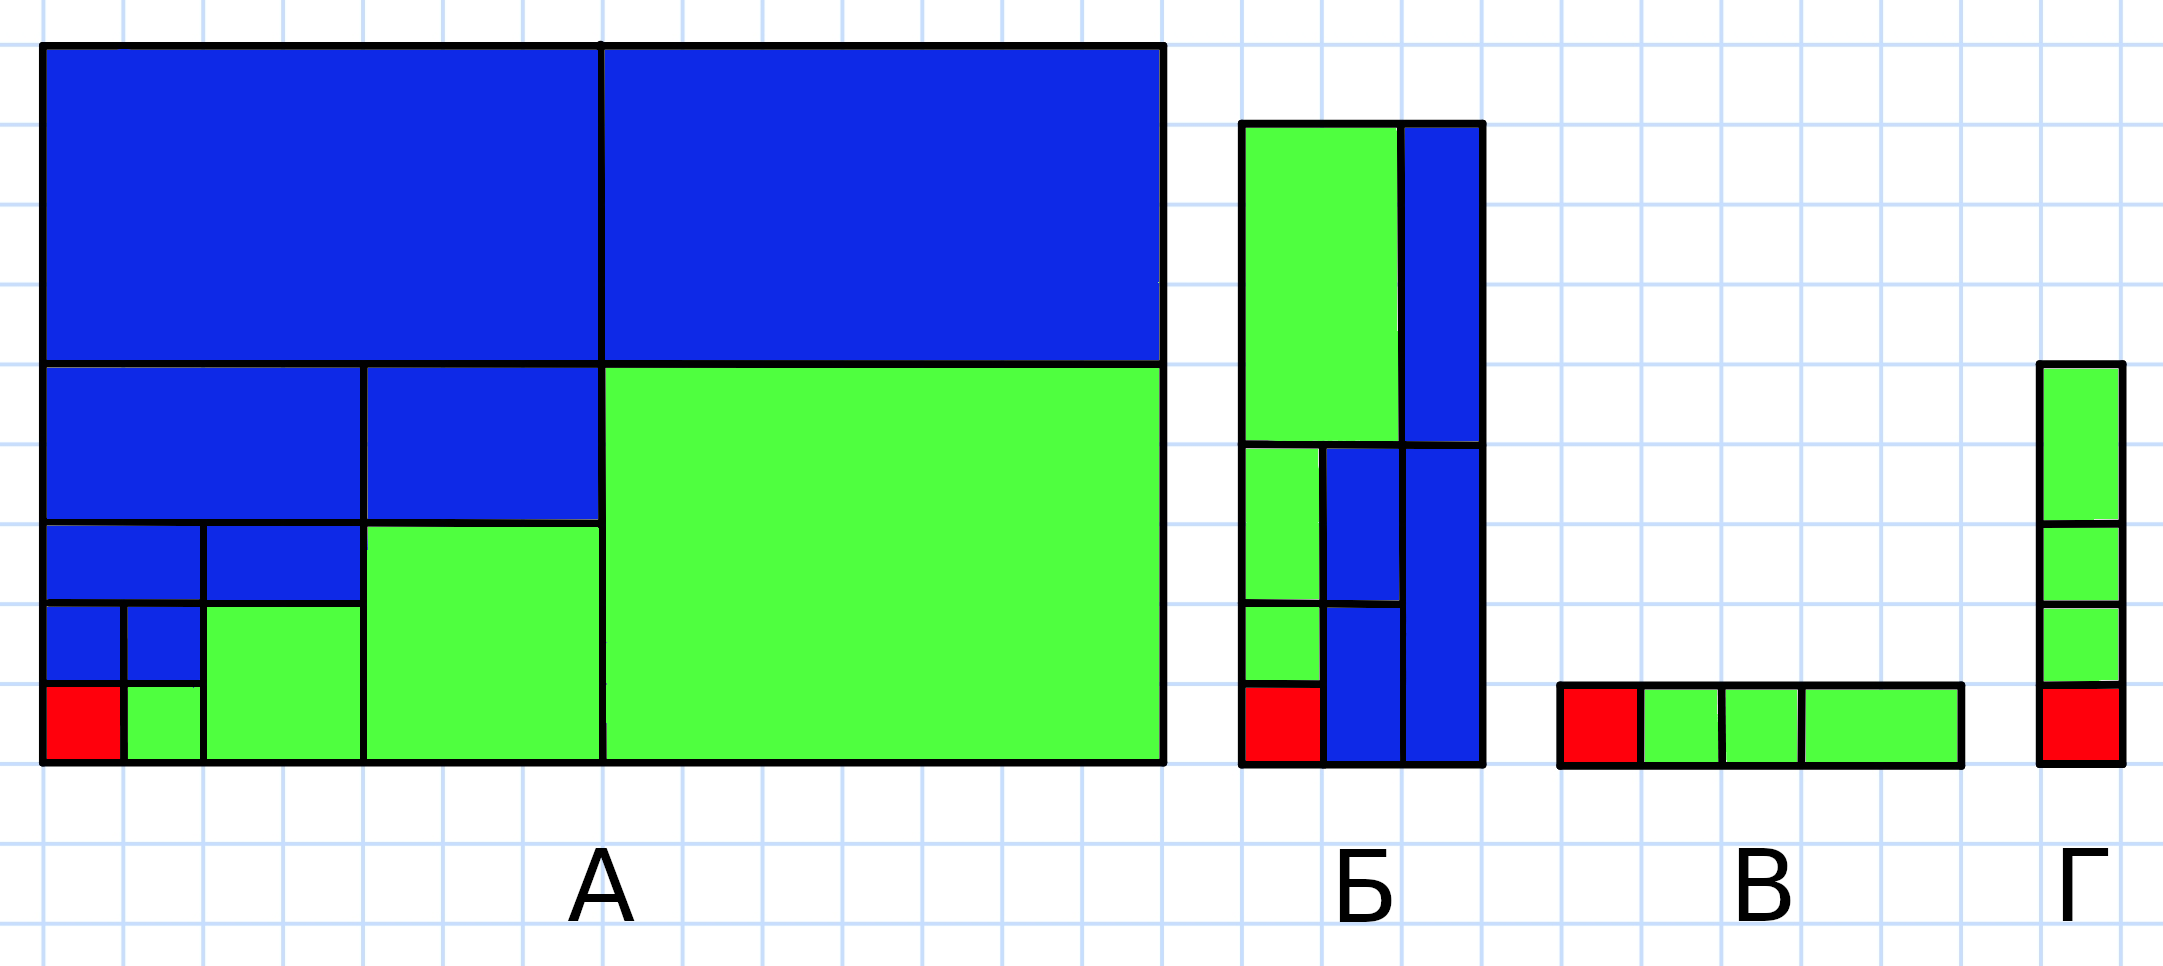
\includegraphics[width=\textwidth ]{img/subdivide_2.png}
	\caption{Примеры разбиения окон в алгоритме Варнока}
	\label{fig:subdivide_2}
\end{figure} 

Подокна, получившиеся в результате разбиения, можно разделить на 3 типа: 

\begin{itemize}
	\item подокна, получившиеся при разбиении окна по стороне с максимальной длиной (в примере отмечены зелёным цветом);
	\item подокна, получившиеся при разбиении окна по стороне с максимальной длиной (в примере отмечены синим цветом);
	\item подокно, имеющее размеры $1\cdot1$ пиксель и являющееся терминатором рекурсии (в примере отмечен красным цветом).
\end{itemize}

Обозначим ширину и высоту исходного окна за $w$ и $h$ соответственно. Тогда максимальное количество разбиений окна по стороне с максимальной длиной будет равно

\begin{equation}
	\label{eq:n_max}
	n_{max} = \lceil\log_{2} (max(w; h))\rceil.
\end{equation}

Количество таких окон будет равно $n_{max}$. Максимальное количество разбиений окна по стороне с минимальной длиной будет равно

\begin{equation}
	\label{eq:n_min}
	n_{min} = \lceil\log_{2} (min(w; h))\rceil.
\end{equation}

Количество таких окон будет равно $2 \cdot n_{max}$. Учитывая единственное подокно, являющееся терминатором рекурсии, максимальный размер стека окон будет равен

\begin{equation}
	\label{eq:res}
	Size = \lceil\log_{2} (max(w; h))\rceil + 2 \cdot \lceil\log_{2} (min(w; h))\rceil + 1.
\end{equation}

%%% Local Variables: 
%%% mode: latex
%%% TeX-master: "rpz"
%%% End: 

\chapter{Алгоритм Варнока}
\label{cha:appendix3}

\begin{figure}[h]
	\centering
	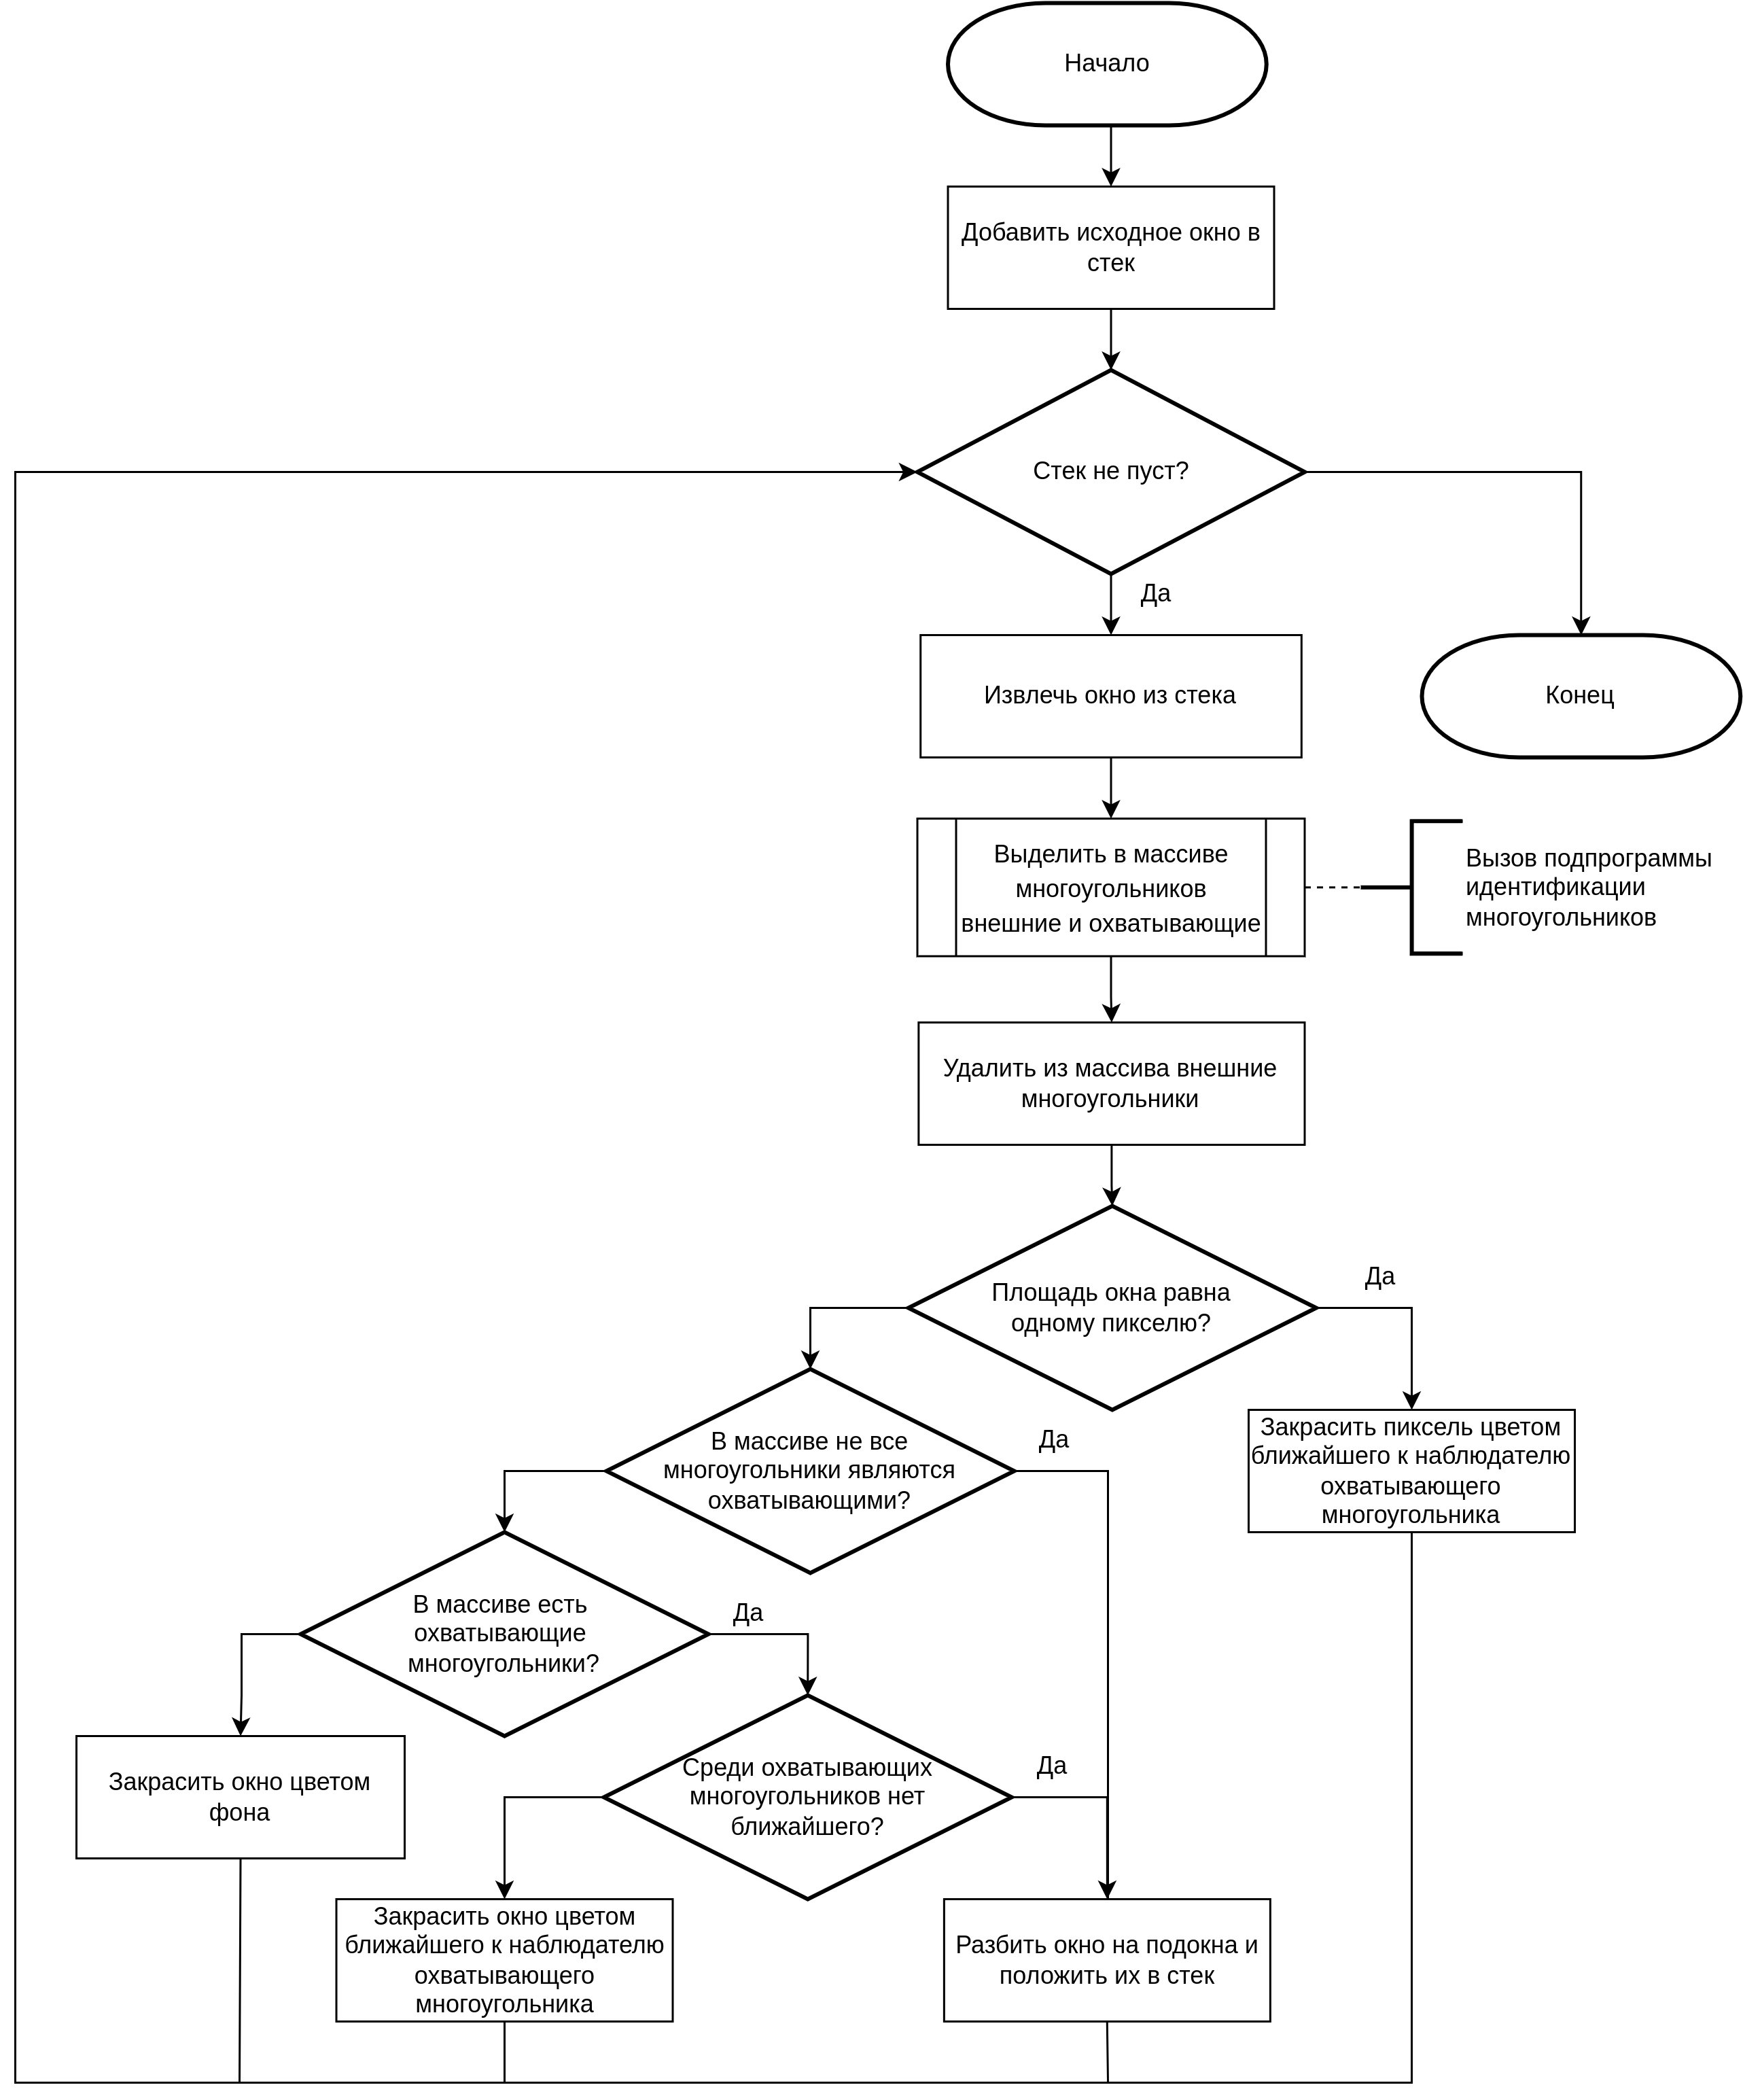
\includegraphics[scale=0.1725 ]{img/flowchart/subdivide3.png}
	\caption{Схема алгоритма Варнока}
	\label{fig:warnock_algorithm}
\end{figure} 

\begin{figure}[h]
	\centering
	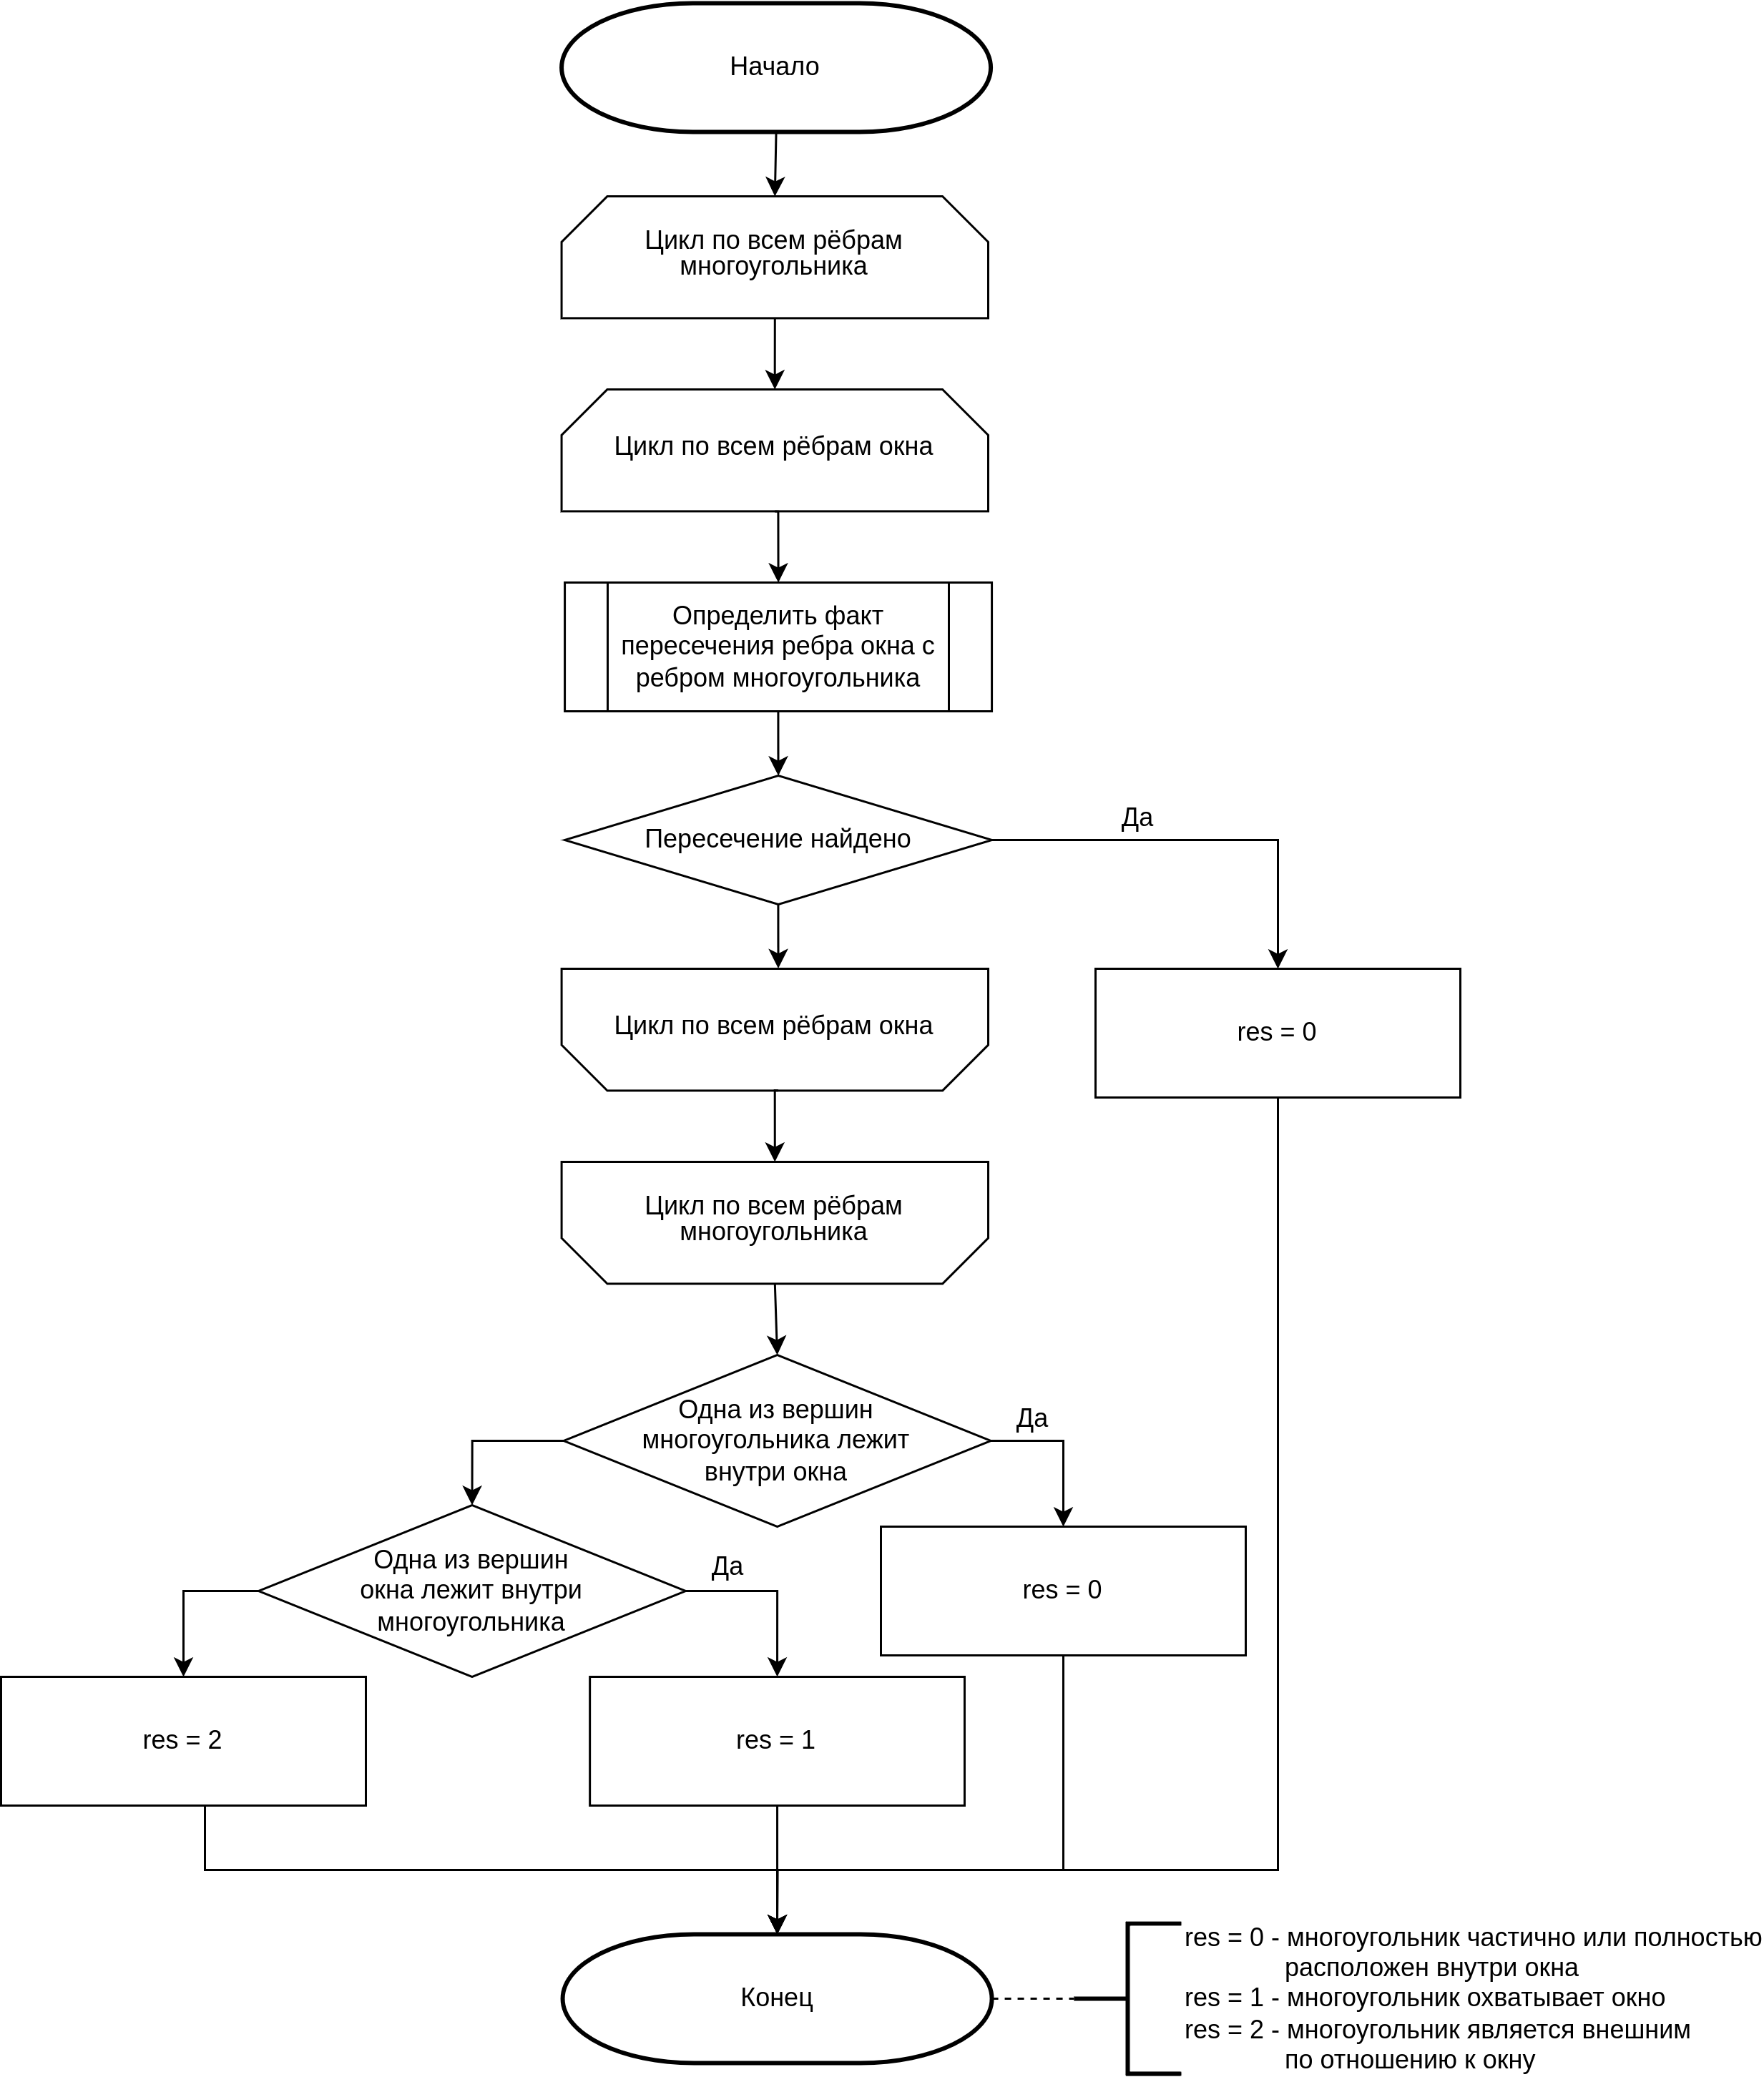
\includegraphics[width=\textwidth ]{img/flowchart/identification2.png}
	\caption{Схема алгоритма определения взаимного расположения многоугольника относительно окна}
	\label{fig:warnock_identification}
\end{figure} 

%%% Local Variables: 
%%% mode: latex
%%% TeX-master: "rpz"
%%% End: 

\chapter{Изображения тестовых моделей}
\label{cha:appendix4}
Разрешение дисплея: 320x240 пикселей.

\begin{figure}[h]
	\centering
	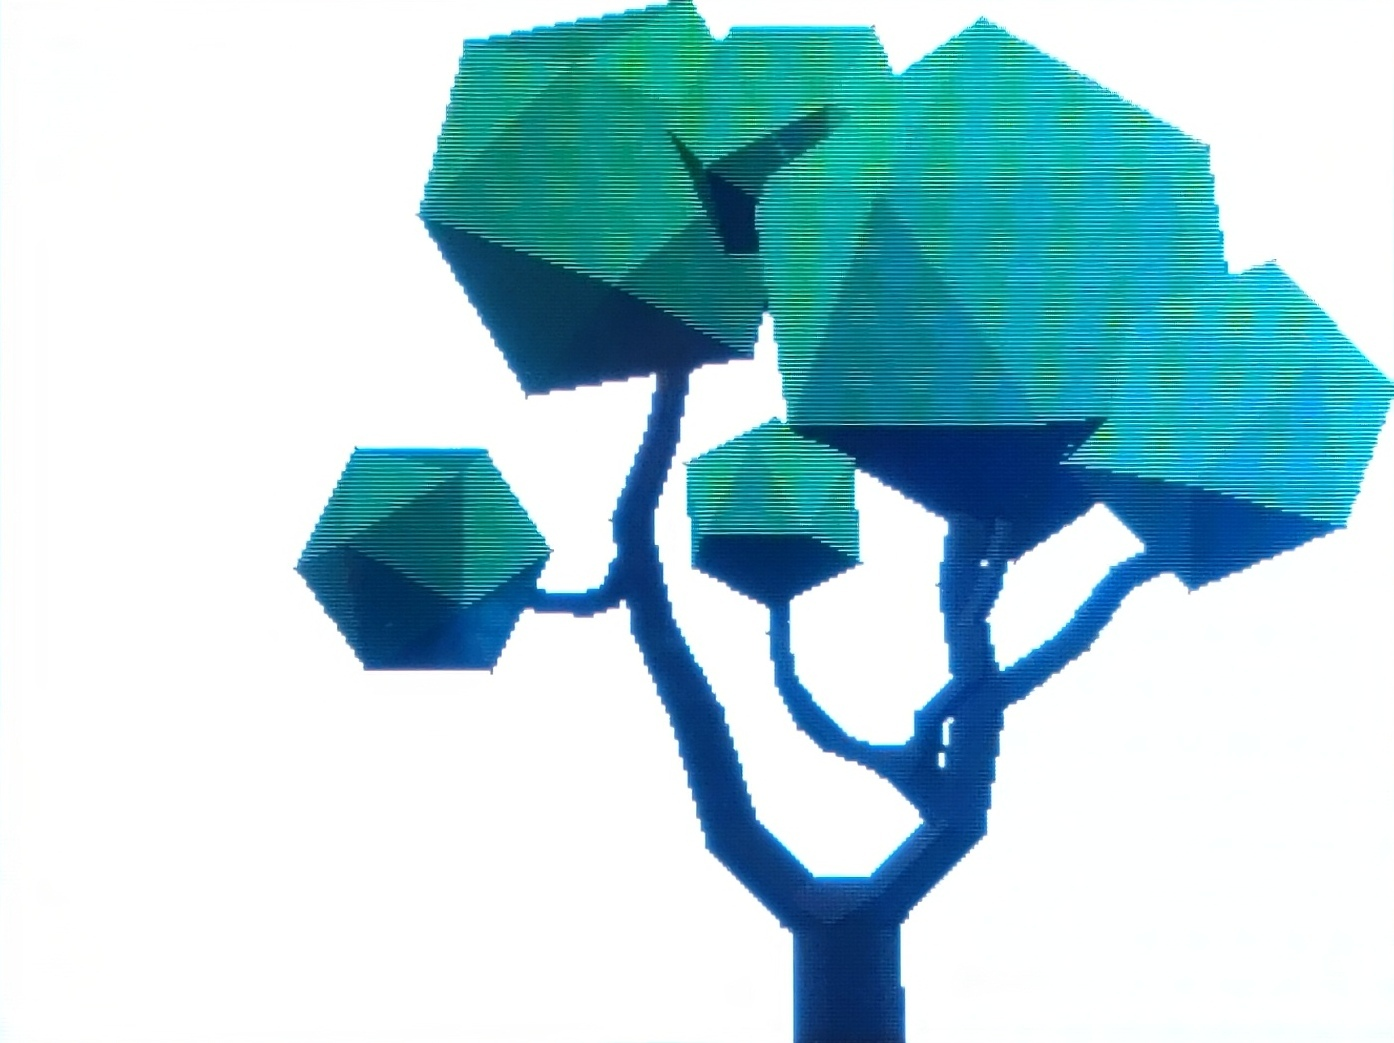
\includegraphics[scale=0.2 ]{img/models/tree.jpg}
	\caption{Модель №1 (312 полигонов).}
	\label{fig:warnock_algorithm}
\end{figure}

\begin{figure}[h]
	\centering
	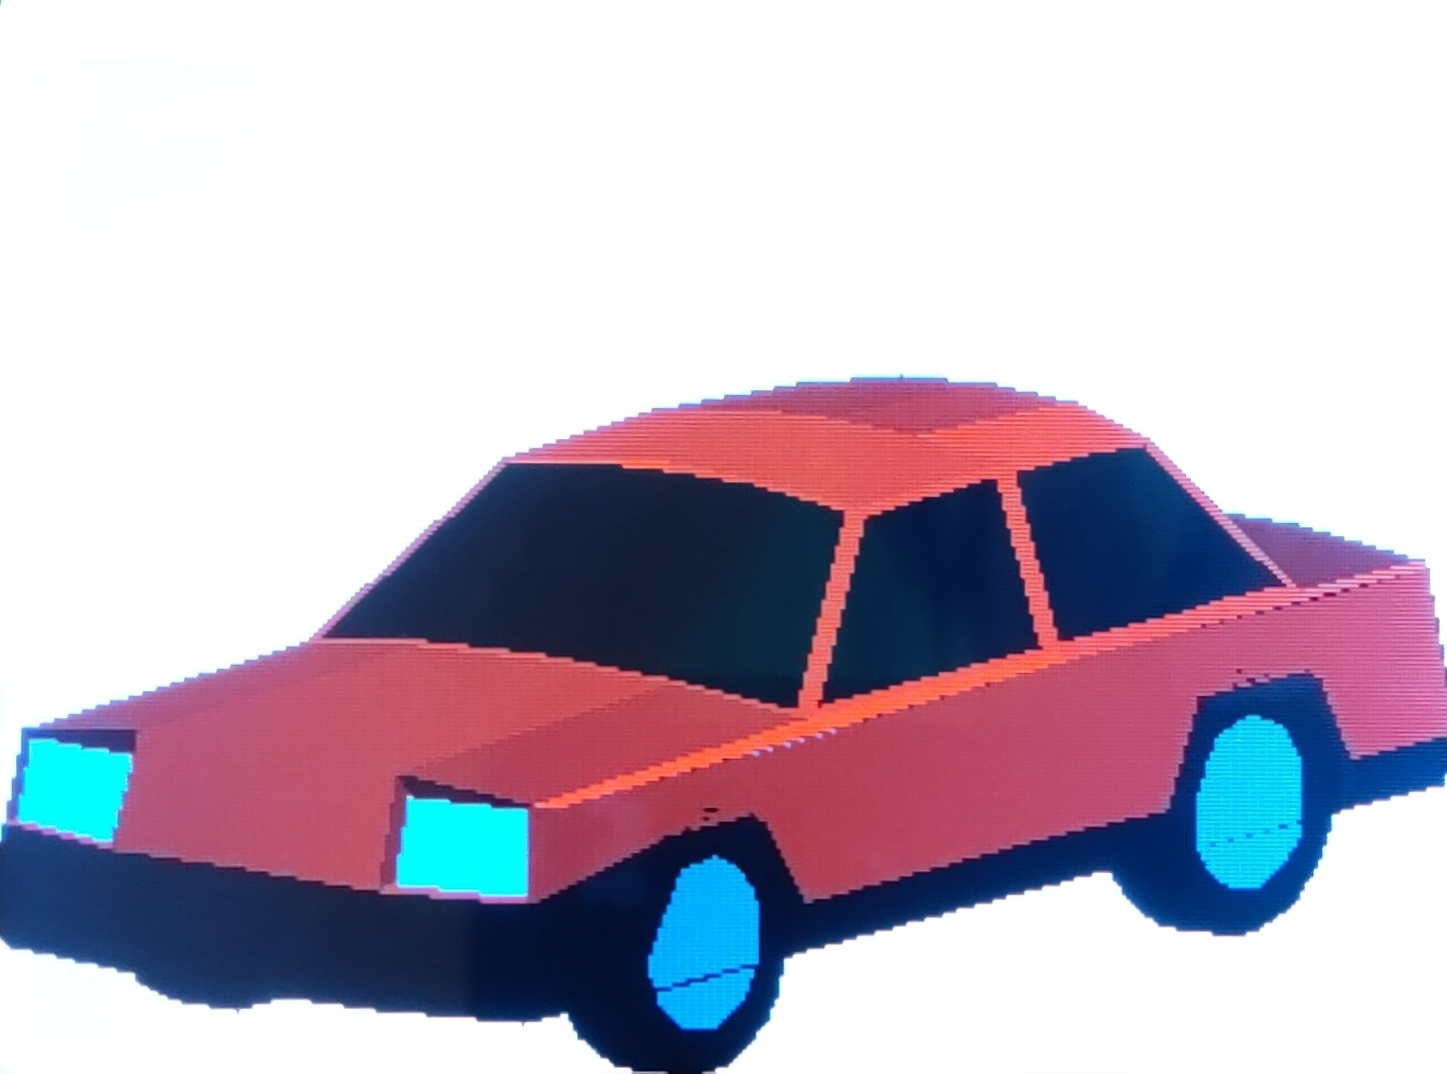
\includegraphics[scale=0.2 ]{img/models/car.jpg}
	\caption{Модель №2 (1172 полигона).}
	\label{fig:warnock_identification}
\end{figure}

\begin{figure}[h]
	\centering
	\vspace*{-9.5cm}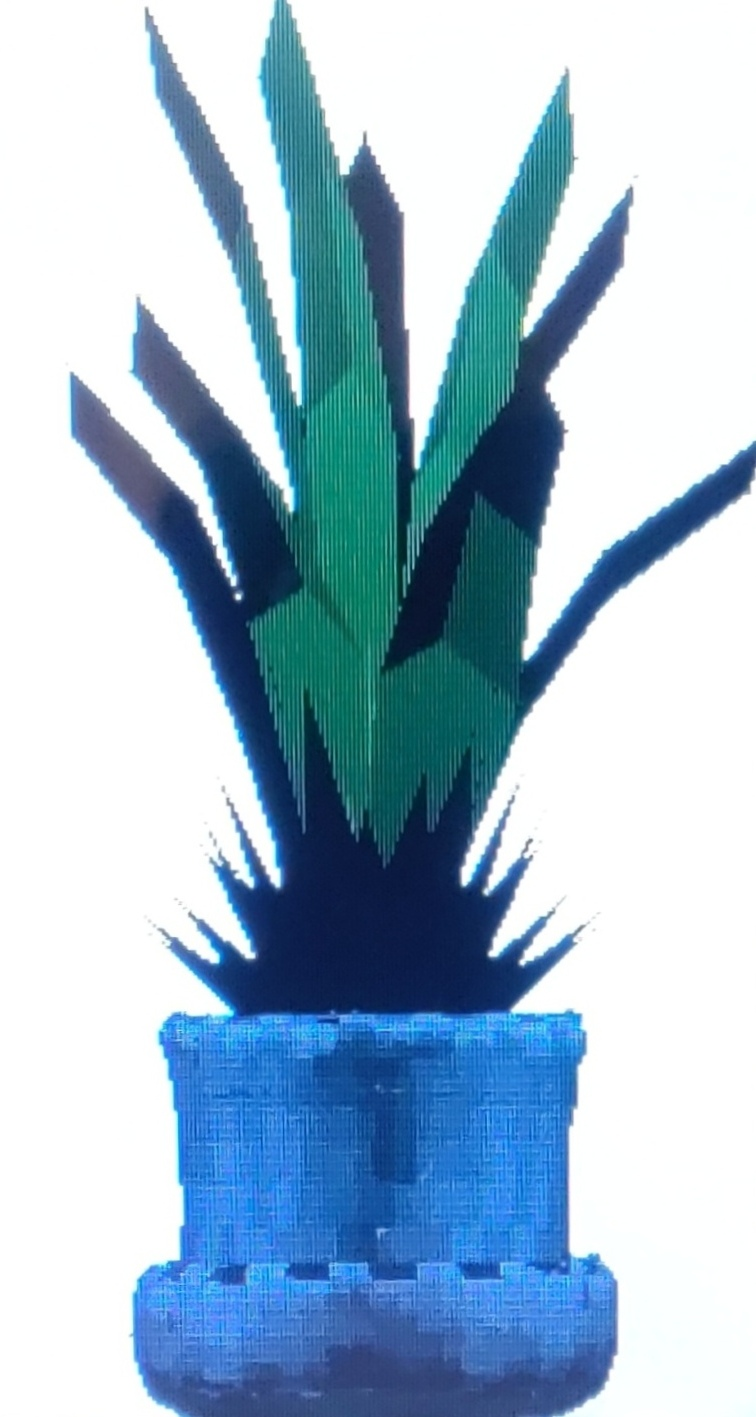
\includegraphics[scale=0.2 ]{img/models/plant.jpg}
	\caption{Модель №3 (6228 полигонов).}
	\label{fig:warnock_identification}
\end{figure}


\end{document}

%%% Local Variables:
%%% mode: latex
%%% TeX-master: t
%%% End:
